\documentclass[a4paper,11pt] {scrartcl}

\addtolength{\textheight}{30mm}
\addtolength{\topmargin}{-10mm}
\addtolength{\textwidth}{20mm}
\addtolength{\oddsidemargin}{-10mm}

\parskip=6pt
\parindent=0pt

\usepackage{setspace,amsmath,listings,xcolor,textcomp,ctable,graphicx,hyperref,dsfont,amssymb,amsthm,subfig,multirow}
\usepackage[numbered]{mcode}
\hypersetup{colorlinks=true, linkcolor=black, citecolor=black, filecolor=black, urlcolor=black}
\graphicspath{{img/}}
\renewcommand{\Pr}{\mathds{P}}
\newcommand \scalemath[2]{\scalebox{#1}{\mbox{\ensuremath{\displaystyle #2}}}}
\newcommand \powers[2] {$\times {#1}^{#2}$}

\title{OD - Mathematics related dissertation}
\subtitle{Determining the optimum vaccination schedule for the MMR vaccine}
\author{667947}

\begin{document}
%Title Page
\maketitle
\thispagestyle{empty}
\begin{abstract}
\doublespacing
An age structured model for measles, mumps and rubella is presented. The model is designed to allow detailed analysis of different vaccination schedules and account for vaccine failure. Parameters for measles, mumps and rubella in the United Kingdom are established and analysis of vaccination against measles is performed. Results with and without waning of vaccine derived immunity are compared. The model shows a dramatic increase in the number of infections occurring when  waning of vaccine derived immunity is included. The cost of a variety of vaccination schedules against measles are compared. All vaccination schedules compared show it is more cost effective to overvaccinate than undervaccinated a population. Without waning of vaccine derived immunity single dose vaccination schemes offer the lowest overall cost. Over a 50 year period, a single dose of vaccine administered at 12 months of age has a total cost of US\$1.916bn(2001) at 85\% coverage and \$1.013bn at 95\% coverage. Whereas, two doses of vaccine at 12 months and at 5 years, has a total cost of \$2.713bn at 85\% coverage and \$1.904bn at 95\% coverage. With waning immunity, both double and triple dose vaccination schedules offer a lower total cost than single dose vaccination schedules. In the 50 year period, a single dose at 12 months is \$5.945bn at 85\% and \$4.804bn at 95\% coverage. Double dose vaccination, with the first dose at 12 months and the second dose at 5 years, has a total cost of \$4.515bn at 85\% coverage and \$2.769bn at 95\% coverage. With a third dose of vaccine at 18 years the total cost is \$4.236bn and \$2.876bn at 85\% and 95\% coverage respectively.
\end{abstract}

%Table of contents
\newpage
\setcounter{page}{1}
\pagenumbering{roman}
\tableofcontents

%Body of text proper
\newpage
\setcounter{page}{1}
\pagenumbering{arabic}
\doublespacing
\section{Introduction}
\label{sec:introduction}
Measles, mumps and rubella (MMR) were all global childhood infections and still affect various parts of the world to different extents. In 1981 there were over $4,000,000$ reported cases of measles worldwide, by 2011 this had reduced to $344,276$ with an estimated $118,000$ deaths\footnote{Under reporting of cases may occur and reporting will be higher for more severe cases which might explain the unexpectedly high ratio of deaths to cases in the reported data.}\cite{whomeasles}. In 2011 there were $726,169$ and $114,449$ reported cases of mumps and rubella worldwide respectively\cite{whoincidencedatabase}. Measles is an infectious viral illness which can cause serious complications such as viral meningitis and pneumonia. It presents with cold-like symptoms, fever, hypersensitivity to light and a rash. If measles is caught during pregnancy, it can be damaging or fatal to the unborn child\cite{nhschoicesmeasles}. Rubella (sometimes referred to as German measles) is a mild viral infection. Symptoms include cold-like symptoms, swollen glands and a red-pink skin rash. If rubella is caught during the first 16 weeks of pregnancy, the unborn child is at serious risk of congenital rubella syndrome (CRS) or death. CRS, discovered by Gregg\cite{gregg1941congenital}, causes severe birth defects including cataracts, blindness, deafness, heart abnormalities and brain damage\cite{nhschoicesrubella}. Mumps is a contagious viral infection and serious complications are rare. It can lead to viral meningitis and swelling of testes/ovaries of post-pubescent individuals. If caught during pregnancy there is a slightly increased chance of miscarriage\cite{nhschoicesmumpscomplications,nhschoicesmumps}. MMR are notifiable diseases\footnote{Registered Medical Practitioners are expected to provide information to the Health Protection Authority (HPA) on incidence of these diseases as part of their professional duties.}\cite{hpanotifiablediseases} in the UK, unpleasant, vaccine preventable and have no cure with treatment only easing symptoms.

The first vaccination, believed to have been invented by Edward Jenner in 1796, was a vaccine against smallpox\cite{stewart2006history}. By 1979 smallpox was the first disease to be eradicated after a global vaccination effort\cite{whosmallpoxfactsheet} and in 2011 Rinderpest, a disease in cattle, became the second\cite{faorinderpesteradication}. For many infectious diseases, when an individual becomes infected, an immune response occurs, the disease is overcome and immunity is acquired. Vaccination bestows immunity without infection hence eliminating the risks of disease, however adverse effects of vaccination do occur. Immunisation reduces the number of infectious individuals within a population, therefore fewer people become infected due to the decreased likelihood of encountering an infectious individual. Eradication can be achieved by vaccination using herd immunity. It is not necessary to vaccinate every individual within a population, immunity must be acquired (via vaccination) by a sufficient number of individuals, so that the basic reproduction number $(R_0)$\footnote{The average number of cases that one infectious case generates over the course of its infectious period when all other individuals within the population are susceptible.} is less than 1. Potential benefits of vaccination include :
\begin{itemize}
\item Eradication - Removes the disease from the global population removing dangers for current and future generations. No further risk and cost of vaccination for future generations.
\item Elimination - Removal of the disease from a regional population. All cases are imported and risk of infection is extremely low. High levels of vaccination must be maintained.
\item Disease control - Lower incidence of disease and risk to population. Reduces likelihood of infection for those vulnerable and high risk individuals who cannot be vaccinated.
\item Cost Reduction - Vaccination can reduce costs for health service providers and society because the vaccine is usually significantly cheaper than the cost of treatment\cite{hinman2004economic,peltola1994elimination}.
\end{itemize}

In addition to benefits, vaccination also has consequences that must be considered before implementation. For example, vaccination can increase the average age of infection in the population. If you were trying to protect pregnant women, then vaccination could exacerbate the problem rather than reducing it (e.g. vaccination against rubella in Greece actually led to the greatest ever number of CRS cases in the 1993\cite{panagiotopoulos1999increase}). In the case of measles, infants of vaccinated mothers have a shorter period of maternal immunity\footnote{The antibodies given to an infant during pregnancy which protect it from diseases for a period of time, called the period of maternal immunity.} in comparison to infants of mothers who have recovered from the disease. Consequently, infants of vaccinated mothers  have a greater period of time between loss of maternal immunity and vaccination (window of susceptibility), which can put them at higher risk of infection\cite{leuridan2010early}.

In 1963 the first vaccine against measles was licensed in the USA\cite{lebaron2007measlespersistence} and in 1968 it was added to the vaccination schedule in the United Kingdom\cite{hpaimmunistationcoverage}. In the United States vaccines for mumps and rubella were licensed in 1967 and 1969 respectively\cite{lebaron2009mumpspersistence,lebaron2009rubellapersistence}. In the UK selective vaccination against rubella began in 1970 in an attempt to reduce the risk of CRS, vaccinating adolescent women. Selective vaccination was ended in 1993\cite{pebody2001seroepidemiology}, 5 years after the introduction of the MMR triple vaccine in 1988\cite{hpaimmunistationcoverage}. Vaccination against mumps was not introduced onto the UK vaccination schedule until the introduction of the MMR vaccine. Initially the MMR vaccine was administered as a single dose\cite{cohen2007vaccine}, but evidence suggested that a high number of measles cases occurred in adolescents who had received a single dose of the vaccine\cite{orenstein2004evolution}, so in 1996 it was recommended that two doses of the MMR vaccine were administered\cite{cohen2007vaccine}. Currently the United Kingdom has a two-dose vaccination schedule for MMR. The first dose (MMR1) is administered at 12--13 months of age and the second dose (MMR2) is administered between 3 and 5 years\cite{nhschoicesvaccinationmmr,nhschoicesvaccinationdates}. In 2010-11 89.7\% of 2 year olds in the UK had received MMR1 and 85\% had received MMR2 by 5 years of age\cite{vaccinationcoverage2011}. In England and Wales prior to vaccination, the number of annual notifications of measles fluctuated between 2--700,000 (see \autoref{mmrnotifications1989} in Appendix). In 1989 there were 26,222, 20,713 and 24,570 notified cases of MMR respectively. By 2009 this had been reduced to 5,191, 18,629 and 1,130 notified cases\cite{hpameaslesnotificationsbyage,hpamumpsnotificationsbyage,hparubellanotificationsbyage} with 1,144, 7,662 and 9 confirmed cases respectively\cite{hpammrconfirmedcases}.

Disease modelling allows us to understand how diseases affect populations, and better understand the effect of vaccination. It allows us to determine the expected impact of a vaccination scheme and make educated decisions on whether the scheme would be beneficial. Crucially, it allows comparison between vaccination schedules and is therefore helpful in determining which schemes offer the greatest benefit. A significant analytical result of modelling is that it helps estimate the proportion of the population that must be vaccinated for eradication\cite{mclean2005mathematical}.

This study compares a variety of vaccination schemes that could be used in the UK and aims to determine a scheme to minimise costs associated with the MMR vaccine. I build a model for measles, mumps and rubella, which allows for detailed analysis of MMR vaccine schedules. I perform a detailed analysis of the results for measles. In particular, I determine the number of infections and vaccinations occurring over a period of time and from this the cost of a vaccination schedule.

\newpage
\section{Building the model}
\label{sec:buildmodel}
\subsection{Aims}
\label{subsec:buildmodelaims}
Since vaccine introduction, disease dynamics have changed. For measles, infants of mothers with vaccine derived immunity have a greater window of susceptibility than infants of recovered mothers. Additionally a large proportion of the population have obtained immunity via vaccination and immunity obtained by vaccination is thought to wane over time\cite{lebaron2007measlespersistence,lebaron2009rubellapersistence,lebaron2009mumpspersistence,davidkin2008persistence}. I aim to assess whether a change in vaccination schedules to account for these factors may be beneficial.

I want to build a model for each disease to allow for the comparison of various vaccination schedules. Numerous types of model could be used: differential, network or stochastic. I use a differential equation model as they can be solved numerically with reasonable accuracy and without a significant amounts of computation. As everything can be thought of as a flow between compartments they are easy to understand. I adapt the standard SIR (Susceptible, Infectious, Recovered) dynamics by adding compartments to account for a variety of additional factors.

I need to measure the impact of a vaccination schedule. Cost is a good measure as there is an associated monetary cost of disease and of administering vaccination. However, immunisation programmes are not simply about minimising cost and can have many aims. Erikson, Wals and Farand\cite{erickson2005analytical} discuss a framework for assessing the success of vaccination scheme, including 58 criteria. Ultimately, decision makers must decide how vaccination effectiveness is measured, allocating weights to different events following vaccination. 

As the model will be used to compare vaccination schedules, it is desirable to  account for the major causes of vaccine failure. Vaccination can fail in one of two ways. Primary vaccination failure is when vaccination does not bestow immunity. Secondary vaccination failure is when immunity is acquired after vaccination but that immunity wanes over time. The main causes of primary vaccination failure in infancy are protective maternal immunity and deficient immune system responses\cite{gans2003measles,glezen2003effect}. I include maternal immunity to account for this, where vaccination is only successful once maternal immunity has been lost. In addition, I do not evaluate vaccination schedules where vaccination occurs before 9 months of age as Gans et al.\cite{gans2003measles} suggests there is no immune response to mumps and measles vaccine before this age.

For measles and mumps, immunity gained through infection is considered lifelong\cite{naniche2009human,hviid2008mumps} and for rubella the likelihood of reinfection is vastly reduced in comparison to vaccination\cite{miller1990rubella}. Waning immunity increases the size of the susceptible population, which can lead to epidemics. In the 2006 mumps epidemic in USA, 51\% of those infected had received 2 doses of MMR vaccine\cite{baum2008cares}. I account for waning of vaccine derived immunity, to allow for a more realistic comparison of vaccination schedules (e.g. with waning immunity can a single vaccination schedule be justified or could a triple vaccination schedule be advocated?).

Crucial to this study is the use of age-stratified modelling. Initially, the model is a system of partial differential equations (PDEs), with time and age as independent variables. More details on age-stratified differential models are given by Anderson\cite{anderson1985age} and Keeling and Rohani\cite{keeling2011modeling}, this study builds on these ideas. I will not deduce analytical results as my model will be too complicated. The PDEs can be solved numerically to obtain the results required.

The model should be capable of comparing vaccination schedules with up to 3 doses. This could be extended to $n$ doses but this is excessive. This allows for comparison of single (offers cost savings compared to double according 667947\cite{mystudy2012} and Carabin\cite{carabin2003future}), double (currently recommended in UK and Pelletier\cite{pelletier1998benefit} suggests more cost effective than single) and triple (not currently used) vaccination schedules. The model includes waning vaccinated immunity and the rate of waning differs according to the number of vaccine doses received. The model must therefore contain 3 vaccinated and 4 susceptible groups. 667947\cite{mystudy2012} uses random vaccination for multiple vaccinations but this overestimates the proportion vaccinated, with $1-(1-p)^i$ proportion of the population vaccinated by the $ith$ dose. In reality, sections of the population will not become vaccinated in spite of encouragement (e.g. some religious groups or objectors). To account for this, those vaccinated receive vaccination at the recommended age(s) and only those who received the $ith$ vaccination dose can receive the $\left(i+1\right)st$ dose.

Maternal immunity protects most infants after birth against MMR for a period of months\cite{leuridan2010early,leuridan2011kinetics,leuridan2012maternal}. For measles, infants born to vaccinated or recovered mothers have differing durations of protective maternal immunity\cite{leuridan2010early}. Consequently I divide those with protective maternal immunity into two groups, those whose mothers were recovered or vaccinated. There is no such evidence for mumps and rubella, although this could be the case. In the case of measles, mothers with low antibody titre give birth to low antibody titre infants\cite{goncalves1999transplacental} hence these infants are often born susceptible or with a short period of protective maternal immunity. So I assume those neither vaccinated nor recovered give birth to susceptible infants. Only those of childbearing age give birth. 

I include an exposed (latent) group, individuals who are infected but not yet infectious. This is a standard extension of the SIR model\cite{anderson1985age,schenzle1984age,levin2011global}. There is evidence of a latent (or incubation) period for MMR\cite{naniche2009human,hviid2008mumps,banatvala2004rubella}. All states included in the model are found in \autoref{tab:modelstatevariables}.

\begin{table} [h]
\centering
\begin{tabular}{c p{55mm} p{85mm}}
\toprule
Symbol & State Name & Description\\
\midrule
$N$ & Population & Entire Population. All states.\\
$M_R$ & Maternal Immunity (Recovered) & Infants with immunity bestowed by mother during pregnancy. Mother recovered from disease.\\
$M_V$ & Maternal Immunity (Vaccinated) & Infants with immunity bestowed by mother during pregnancy. Mother vaccinated against disease.\\
$S_{i}$& Susceptible - $i$th dose received &Individuals could become exposed on contact with infected individuals. Vaccinated $i$ times, but for $i>0$ their immunity has waned.\\
$V_{i}$& Vaccinated - $i$th dose received& Individuals have vaccine derived immunity to the disease. Has received $i$ doses of vaccine. \\
$E$& Exposed (Latent) & Individuals infected by the disease but not yet infectious to other individuals.\\
$I$& Infectious & Individuals infected by the disease and infectious to others. If they come into contact with susceptible individuals they can transmit the disease. \\
$R$& Recovered & Individuals who had the disease and have immunity from future infection. \\
\bottomrule
\end{tabular}
\caption{Model state variables}
\label{tab:modelstatevariables}
\end{table}

\subsection{Assumptions}
\label{subsec:buildmodelassumptions}
Based on the aims given in \autoref{subsec:buildmodelaims} I build an age-stratified model of the diseases as a system of PDEs. The parameters used in the model can be found in \autoref{tab:parameters}.

\begin{table}[h]
\centering
\begin{tabular}{c p{11.5cm}}
\toprule
Symbol & Parameter\\
\midrule
$a$ & Age \\
$t$ & Time \\
$\alpha (a)$ & Death rate. Age dependent.\\
$\beta (a_1,a_2)$ & Transmission rate. Age dependent.\\
$\kappa$ & Transmission risk. Constant.\\
$C (a_1,a_2)$ & Contact rate. Age dependent.\\
$\delta (a)$ & Decay rate of vaccinated maternal immunity. Age dependent\\
$\epsilon (a)$ & Decay rate of recovered maternal immunity. Age dependent\\
$\psi _i (a)$ & Waning rate of vaccinated immunity after $ith$ dose. Age dependent.\\
$\phi_i(a)$ & Vaccination gate function. Proportion entering $S_i$ after losing maternal immunity. Age dependent.\\
$\rho_i(a)$ & $ith$ dose uptake. Proportion of those who received $\left(i-1\right)st$ vaccination dose that receive $ith$ dose. Age dependent.\\
$\sigma$ & Progression rate. Constant.\\
$\gamma$ & Recovery rate. Constant.\\
$l$ & Lower bound of childbearing age range. Constant.\\
$u$ & Upper bound of childbearing age range. Constant.\\
$\tau(t)$ & Birth density. Time dependent.\\
\bottomrule
\end{tabular}
\caption{PDE model parameters}
\label{tab:parameters}
\end{table}

The model represents the following assumptions.
\begin{itemize}
%Population
\item{Death rate is age dependent, at rate $\alpha (a)$.}
\item{Infection does not cause death.}
\item{The generation of individuals aged zero is time dependent $\tau \left(t \right)$.}
\item{Stable population size. Deaths are equal to births at any time $t$ (i.e. $\int^{\infty}_{0} \alpha(a) N(a,t) da = \tau (t)$).}
\item{Only those in the childbearing age range give birth. Lower age bound $l$. Upper age bound $u$.}
\item{Entire childbearing age range give birth (i.e. no distinction between males and females).}
\item{Those recovered ($R$) of childbearing age give birth into $M_R$ and $S_0$. $\left(1-\epsilon(0)\right)$ proportion of births enter $M_R$. $\epsilon(0)$ proportion of births enter $S_0$.}
\item{Those vaccinated ($V_i$) of childbearing age give birth into $M_V$ and $S_0$. $\left(1-\delta(0)\right)$ proportion of births enter $M_V$. $\delta(0)$ proportion of births enter $S_0$.}
\item{Those of childbearing age not recovered or vaccinated give birth into $S_0$.}
\item{Geographically homogeneous mixing. Transmission is not location dependent.}
%Disease Behaviour
\item{No interference between infections.}
\item{Contacts occur according $C(a_1,a_2)$, the rate of contact of an individual from age group $a_2$ has with those in age group $a_1$.}
\item{Transmission risk $\kappa$, the likelihood of successful transmission. When a susceptible individual comes into contact with an infectious individual, they have probability $\kappa$ of becoming exposed.}
\item{Transmission rate $\beta (a_1,a_2)$. Rate of disease transmission from age group $a_1$ into age group $a_2$. $\beta = \kappa C$}
\item{Progression rate, at which exposed individuals become infectious, is constant $\sigma$.}
\item{Recovery rate, at which infectious individuals become recovered, is constant $\gamma$.}
%Vaccination assumptions
\item{Vaccination is successful on susceptible or vaccinated individuals. Those in $S_i$ or $V_i$ enter $V_{i+1}$.}
\item{Vaccination doses are applied at a recommended age $a$. Initial dose is applied to $\rho_1$ of entire population at $a_1$. The $(i+1)st$ dose is applied at $a_{i+1}$ to $\rho_{i+1}$ of those in $S_i$ or $V_i$ and $\prod^{i+1}_{k=1} \rho_{k}$ of those in $M_R$ or $M_V$.}
%Immunity Assumptions
\item{Vaccinated immunity wanes, those in $V_i$ enter $S_i$. Waning is age-dependent at rate $\psi_i (a)$.}
\item{Immunity after recovery from disease is lifelong}
\item{Vaccination fails if an infant has maternal immunity (i.e. in $M_R$ or $M_V$).}
\item{Vaccination does not alter maternal immunity.}
\item{When maternal immunity ($M_R$ or $M_V$) is lost individuals become susceptible. Those who have received $i$ doses of vaccination enter $S_i$.}
\item{Maternal immunity is lost from $M_R$ and $M_V$ at age-dependent rates $\epsilon (a)$ and $\delta (a)$ respectively.}
\item{Vaccination fails when it is applied to those with maternal immunity. When individuals who had received $i$ doses of vaccination lose maternal immunity they enter $S_i$. The age-dependent \textit{vaccination gate function} $\phi_i(a)$ `remembers'\ the proportion of infants with maternal immunity who have received $i$ doses of vaccination at age $a$ (see \autoref{fig:establishingparametersgatefunctionexample}).}
\end{itemize}

\begin{figure}[hp]
\centering
\includegraphics[width=120mm]{gatefunctionexample}
\caption{Vaccination gate function example. The first dose of vaccine is administered to 95\% of the population at 1 year of age and the second dose is administered at 5 years of age to 80\% of those who received the first dose of vaccine. Consequently the proportion of the population that have received one dose of vaccine between 1--5 years of age is 95\% and from 5 years of age onwards is 19\%. The proportion of the population that have received two doses of vaccine from 5 years of age onwards is 76\%.}
\label{fig:establishingparametersgatefunctionexample}
\end{figure}

\singlespacing
\subsection{PDE model}
\label{subsec:buildmodelpdemodel}
\begin{align*}
&\frac{\partial M_V}{\partial t}(a,t) = -\left[\delta(a)+\alpha(a) \right]M_V(a,t) - \frac{\partial M_V}{\partial a}(a,t)\\
&\frac{\partial M_R}{\partial t}(a,t) = -\left[\epsilon(a)+\alpha(a) \right]M_R(a,t) - \frac{\partial M_R}{\partial a}(a,t)\\
&\frac{\partial S_0}{\partial t}(a,t) = \left(1-\sum_{i=1}^3 \phi_i(a)\right)\left[\delta(a)M_V(a,t) + \epsilon(a)M_R(a,t)\right] - \left[\rho_1(a) + \lambda(a,t) + \alpha(a) \right]S_0(a,t)- \frac{\partial S_0}{\partial a}(a,t) \\
&\frac{\partial S_1}{\partial t}(a,t) = \phi_1(a)\left[\delta(a)M_V(a,t) + \epsilon(a)M_R(a,t)\right] + \psi_1V_1(a,t)- \left[\rho_{2}(a) + \lambda(a,t) + \alpha(a) \right]S_1(a,t)- \frac{\partial S_1}{\partial a}(a,t)\\
&\frac{\partial S_2}{\partial t}(a,t) = \phi_2(a)\left[\delta(a)M_V(a,t) + \epsilon(a)M_R(a,t)\right] + \psi_2V_2(a,t)- \left[\rho_{3}(a) + \lambda(a,t) + \alpha(a) \right]S_2(a,t)- \frac{\partial S_2}{\partial a}(a,t)\\
&\frac{\partial S_3}{\partial t}(a,t) = \phi_3(a)\left[\delta(a)M_V(a,t) + \epsilon(a)M_R(a,t)\right]+ \psi_3V_3(a,t) - \left[\lambda(a,t) + \alpha(a) \right] S_3(a,t)- \frac{\partial S_3}{\partial a}(a,t)\\
&\frac{\partial V_{1}}{\partial t}(a,t) = \rho_{1}(a)S_{0}(a,t) - \left[ \psi_{1}(a) + \rho_{2}(a) + \alpha(a) \right]V_{1}(a,t) - \frac{\partial V_{1}}{\partial a}(a,t)\\
&\frac{\partial V_{2}}{\partial t}(a,t) = \rho_{2}(a)\left[S_{1}(a,t)+V_{1}(a,t)\right] - \left[ \psi_{2}(a) + \rho_{3}(a) + \alpha(a) \right]V_{2}(a,t) - \frac{\partial V_{2}}{\partial a}(a,t)\\
&\frac{\partial V_{3}}{\partial t}(a,t) = \rho_{3}(a)\left[S_{2}(a,t)+V_{2}(a,t)\right] - \left[ \psi_{3}(a) + \alpha(a) \right]V_{3}(a,t) - \frac{\partial V_{3}}{\partial a}(a,t)\\
&\frac{\partial E}{\partial t}(a,t) =\lambda(a,t)\sum_{i=0}^3{S_i}(a,t) - \left[\sigma + \alpha(a)\right]E(a,t)- \frac{\partial E}{\partial a}(a,t)\\
&\frac{\partial I}{\partial t}(a,t) = \sigma E(a,t) -\left[\gamma + \alpha(a)\right]I(a,t) - \frac{\partial I}{\partial a}(a,t)\\
&\frac{\partial R}{\partial t}(a,t) = \gamma I(a,t) - \alpha(a)R(a,t) - \frac{\partial R}{\partial a}(a,t)
\end{align*}
\textbf{where}
\begin{align*}
&N(a,t) = M_V(a,t) + M_R(a,t) + \sum_{i=0}^3 S_i(a,t) + \sum_{i=1}^3 V_i(a,t) + E(a,t) + I(a,t) + R(a,t)\\
&\lambda(a,t) = \int_0^\infty \beta (\hat{a},a)\frac{I(\hat{a},t)}{N(\hat{a},t)} \mathrm{d}\hat{a}\\
&\frac{\partial N}{\partial t}(a,t) = -\alpha(a) N(a,t) - \frac{\partial N}{\partial a}(a,t)
\end{align*}
\textbf{Boundary Conditions}\\
\textbf{for} $1\leq q \leq 3$ 
\begin{align*}
 &M_V(0,t) = \tau(t) \frac {\left(1-\delta(0)\right) B_V(t)} {B_N(t)}
 \qquad M_R(0,t) = \tau(t)\frac {\left(1-\epsilon(0)\right) B_R(t)} {B_N(t)}\\
 &S_0(0,t) = \tau(t) \frac {\left(\delta(0)-1\right) B_V(t) + \left(\epsilon(0)-1\right) B_R(t) + B_N(t)} {B_N(t)}\\
 &E(0,t) = I(0,t) = R(0,t) = V_q(0,t) = S_q(0,t) = 0 
 \end{align*}
 \textbf{where}
\begin{equation*}
\tau(t) = \int_{0}^{\infty} \alpha (a)N(a,t) \mathrm{d}a
\quad B_V(t) = \sum^{3}_{i =1}\int_{l}^{u} V_{i}(a,t) \mathrm{d}a
\quad B_R(t) = \int_{l}^{u} R(a,t) \mathrm{d}a
\quad B_N(t) = \int_{l}^{u} N(a,t) \mathrm{d}a
\end{equation*}

\newpage
\doublespacing
It is simpler to think of the system of PDEs as a diagram of flows between compartments (see \autoref{fig:pdediseasemodel}). Ageing and death are not included within this diagram but can be thought of as a constant flow. Vaccination is applied to the appropriate proportion of the population at each age. It is successful for those who are in the susceptible or vaccinated groups. It would fail for those within other groups, in particular those with maternal immunity. Consequently, those who have maternal immunity, when they are vaccinated remain within the maternal immunity group. Due to the \textit{vaccination gate functions} $\phi_i$ when protective maternal immunity is then lost they then enter the susceptible group corresponding to however many doses of vaccination they have received.
\begin{figure}[h]
\centering
\includegraphics[width=\textwidth]{modelflow.jpg}
\caption{Diagram of the PDE model. $\phi_i$ are the age dependent gate functions described in \autoref{fig:establishingparametersgatefunctionexample}}
\label{fig:pdediseasemodel}
\end{figure}

\subsection{Discretisation}
\label{subsec:buildmodeldiscretisation}
There are numerous ways to numerically solve a system of PDEs. A Runge-Kutta 4th order scheme is desirable, as it offers good accuracy and run time. It is considered the standard numerical solver for ordinary differential equations(ODEs) for small step size $h$. However as Runge-Kutta solves ODE systems, it is not appropriate for the model as described in \autoref{subsec:buildmodelpdemodel}. One method is to approximate the PDE model with an ODE model, then Runge-Kutta can be applied.

I combine similar methods, using ideas from Schenzle\cite{schenzle1984age}, Keeling and Rohani\cite{keeling2011modeling} and Levin\cite{levin2011global}. I discretise the ODE model utilising the idea of cohorts used by Schenzle\cite{schenzle1984age}, having birth month cohorts instead of school year cohorts. I can model the decay of protective maternal immunity using a discretised maternal immunity function. Using birth month cohorts allows vaccination to be applied to a cohort at very specific ages. I follow the cohorts for $m$ months, calling these age groups $1,2, \dots ,m$. These birth cohorts will shift (or age) every month. Those that leave age group $m$ are then added into age group $m+1$. After birth cohorts I have age groups of some width, in total $n$ of these age groups, call them $m+1,m+2, \dots, m+n$. Within these groups age is modelled as a flow with parameter $\omega(i)$, corresponding to the ageing parameter of age group $i$. They will contain those beyond the age of vaccination and loss of maternal immunity. For $a,b \in \left\lbrace j | 1\leq j \leq \left(m+n\right)\right\rbrace$, age group $a$ contains all individuals aged $l$ and age group $b$ contains the oldest individuals less than $u$ years. Let $x$ be some state, let $j$ be some age group where $ 1\leq j \leq \left(m+n\right)$ and let $t$ be the time. Then $x(j,t)$ denotes the those individuals contained within the state $x$ of age group $j$ at time $t$. We can approximate the PDE model given in \autoref{subsec:buildmodelpdemodel} as ODEs and discrete events, a summary of which events are discrete and which events occur within the ODEs can be found in \autoref{tab:modelevents}.

\begin{table} [h]
\centering
\begin{tabular}{l l}
\toprule
System of ODEs & Discrete events\\
\midrule
Birth & Loss of maternal immunity\\
Death & Vaccination gate functions\\
Infection & Vaccination\\
Waning of vaccinated immunity & Resetting birth group to 0\\
Progression & Ageing up to $m$ months\\
Recovery &  \\
Ageing above $m$ months &\\
\bottomrule
\end{tabular}
\caption{Summary of the events occurring within the discretised model}
\label{tab:modelevents}
\end{table}

\subsubsection{Discrete events}
\label{subsubsec:buildmodeldiscreteevents}
I model some events discretely. Shifting age cohorts is a discrete event that occurs every month. Vaccination and decay of maternal immunity are discrete events. Discrete events all occur at the same time, vaccination and waning of maternal immunity only occur at given ages. By choosing $\phi_i$ appropriately, those who lose maternal immunity after the $ith$ dose of vaccination enter $S_i$, the susceptible but vaccinated group. Those individuals who lose maternal immunity the same month that they receive the $ith$ dose of vaccination enter $S_i$.

\singlespacing
\textbf{for} $q = 1,2,3$
\begin{equation*}
{M_V}(1,t) =
{M_R}(1,t) =
{S_0}(1,t) =
{S_q}(1,t) =
{V_q}(1,t) =
{E}(1,t) =
{I}(1,t) =
{R}(1,t) = 0
\end{equation*}
\textbf{for} $j = 2, \dots , m$
\begin{align*}
&{M_V}(j,t) = \left[1-\delta(j)\right]{M_V}(j-1,t) \qquad
{M_R}(j,t) = \left[1-\epsilon(j)\right]{M_R}(j-1,t)\\
&{S_0}(j,t) = \left[ 1 - {\rho_{1}}(j) \right] {S_0}(j-1,t) + \left[ 1 - {\phi_1}(j) - {\phi_2}(j) - {\phi_3}(j)\right]\left[ \delta(j) {M_V}(j-1,t) + \epsilon(j) {M_R}(j-1,t)\right]\\
&{S_1}(j,t) = \left[ 1 - {\rho_{2}}(j) \right] {S_1}(j-1,t) + {\phi_1}(j) \left[ \delta(j) {M_V}(j-1,t) + \epsilon(j) {M_R}(j-1,t)\right]\\
&{S_2}(j,t) = \left[ 1 - {\rho_{3}}(j) \right] {S_2}(j-1,t) + {\phi_2}(j) \left[ \delta(j) {M_V}(j-1,t) + \epsilon(j) {M_R}(j-1,t)\right]\\
&{S_3}(j,t) = {S_3}(j-1,t) + {\phi_3}(j) \left[ \delta(j) {M_V}(j-1,t) + \epsilon(j) {M_R}(j-1,t)\right]\\
&{V_1}(j,t) = \left[ 1 - {\rho_{2}}(j) \right]{V_1}(j-1,t) + {\rho_{1}}(j) {S_0}(j-1,t)\\ 
&{V_2}(j,t) = \left[ 1 - {\rho_{3}}(j) \right]{V_2}(j-1,t) + {\rho_{2}}(j) \left[{S_1}(j-1,t)+{V_1}(j-1,t)\right]\\
&{V_3}(j,t) = {V_3}(j-1,t) + {\rho_{3}}(j) \left[{S_2}(j-1,t)+{V_2}(j-1,t)\right]\\
&E(j,t) = E(j-1,t) \qquad
I(j,t) = I(j-1,t) \qquad
R(j,t) = R(j-1,t)
\end{align*}
\begin{align*}
&{M_V}(m+1,t) = {M_V}(m+1,t)+{M_V}(m,t)& \quad
&{M_R}(m+1,t) = {M_R}(m+1,t)+{M_R}(m,t)\\
&{S_0}(m+1,t) = {S_0}(m+1,t)+{S_0}(m,t)& \quad
&{S_1}(m+1,t) = {S_1}(m+1,t)+{S_1}(m,t) \\
&{S_2}(m+1,t) = {S_2}(m+1,t)+{S_2}(m,t)& \quad
&{S_3}(m+1,t) = {S_3}(m+1,t)+{S_3}(m,t)\\
&{V_1}(m+1,t) = {V_1}(m+1,t)+{V_1}(m,t)& \quad
&{V_2}(m+1,t) = {V_2}(m+1,t)+{V_2}(m,t) \\
&{V_3}(m+1,t) = {V_3}(m+1,t)+{V_3}(m,t)& \quad
&{E}(m+1,t) = {E}(m+1,t)+{E}(m,t) \\
&{I}(m+1,t) = {I}(m+1,t)+{I}(m,t) & \quad
&{R}(m+1,t) = {R}(m+1,t)+{R}(m,t)
\end{align*}

\newpage
\subsubsection{ODE model}
\label{subsubsec:buildmodelodemodel}
Newborns $M_V$,$M_R$ and $S_0$.
\begin{align*}
\frac{dM_V}{dt}(1,t) &= \tau(t) \left[1-\delta(1)\right] \frac{B_V(t)}{B_N(t)} - \alpha(1) {M_{V}}(1,t)\quad
\frac{dM_R}{dt}(1,t) = \tau(t) \left[1-\epsilon(1)\right] \frac{B_R(t)}{B_N(t)} - \alpha(1) {M_R}(1,t)\\
\frac{dS_0}{dt}(1,t) &= \tau(t) \left[\frac{B_N(t)+\left(\delta (1) -1\right)B_V(t)+\left(\epsilon (1) -1\right)B_R(t)}{B_N(t)}\right] - \left[ \lambda(1,t) + \alpha(1) \right]S_0(1,t)
\end{align*}
\textbf{for} $2\leq j \leq m$. Other young individuals $M_V$,$M_R$ and $S_0$.
\begin{equation*}
\frac{dM_V}{dt}(j,t) = - \alpha(j) M_V (j,t)\quad
\frac{dM_R}{dt}(j,t) = - \alpha(j) M_R (j,t)\quad
\frac{dS_0}{dt}(j,t) = - \left[ \lambda(j,t) + \alpha(j) \right]S_0(j,t)
\end{equation*}
\textbf{for} $1\leq j \leq m$ and $q = 1,2,3$. Young individuals not $M_V$,$M_R$ or $S_0$ up to age group $m$.
\begin{align*}
&\frac{dS_q}{dt}(j,t) = {\psi_q}(j){V_{q}(j,t)} - \left[\lambda(j,t) + \alpha(j) \right]S_q(j,t) \quad &
&\frac{dV_q}{dt}(j,t) = -\left[ {\psi_q}(j) + \alpha(j)\right]{V_q}(j,t) \\
&\frac{dE}{dt}(j,t) = \lambda(j,t) \sum^3_{k=0} S_k(j,t) - \left[ \sigma + \alpha(j) \right]E(j,t) \quad &
&\frac{dI}{dt}(j,t) = \sigma E(j,t) - \left[ \gamma + \alpha(j) \right]I(j,t) \\
&\frac{dR}{dt}(j,t) = \gamma I(j,t) - \alpha(j) R(j,t) 
\end{align*}
\textbf{for} $m+1\leq j \leq m+n$ and $q = 1,2,3$. Ageing occurs as a flow. For the first older age group, $m+1$ there is no ageing decay into this group as occurs at discrete events so $\omega(m) = 0$. The middle older age groups are the same. The oldest group is infinitely wide and no longer ages so $\omega(m+n) = 0$.
\begin{align*}
&\frac{dM_V}{dt}(j,t) = \omega(j-1)M_{V}(j-1,t) - \left[\alpha(j)+\omega(j)\right] M_V(j,t)\\
&\frac{dM_R}{dt}(j,t) = \omega(j-1)M_{R}(j-1,t)- \left[\alpha(j)+\omega(j)\right] M_R(j,t) \\
&\frac{dS_0}{dt}(j,t) = \omega(j-1)S_{0}(j-1,t)- \left[\lambda(j,t)+ \alpha(j)+ \omega(j) \right]S_0(j,t) \\
&\frac{dS_q}{dt}(j,t) = \omega(j-1)S_{q}(j-1,t)+ {\psi_q}(j){V_{q}}(m,t) - \left[\lambda(j,t)+ \alpha(j)+ \omega(j) \right]{S_{q}}(j,t) \\
&\frac{dV_q}{dt}(j,t)= \omega(j-1)V_{q}(j-1,t)-\left[\psi_q(j) + \alpha(j) + \omega(j)\right]{V_{q}}(j,t) \\ 
&\frac{dE}{dt}(j,t) = \omega(j-1)E(j-1,t)+\lambda(j,t) \sum^3_{k=0} S_{k}(j,t) - \left[ \sigma + \alpha(j) + \omega_(j) \right]E(j,t) \\
&\frac{dI}{dt}(j,t) = \omega(j-1)I(j-1,t)+\sigma E(j,t) - \left[ \gamma + \alpha(j) + \omega(j) \right]I(j,t) \\
&\frac{dR}{dt}(j,t) = \omega(j-1)R(j-1,t)+\gamma I(j,t) - \left[ \alpha(j) + \omega(j) \right] R(j,t)
\end{align*}
\textbf{where}
\begin{align*}
\lambda(j,t) &= \sum^{m+n}_{k=1} \frac{\beta(k,j) I(k,t)}{N(k,t)} \quad 
\tau (t)= \sum^{m+n}_{k=1} \alpha(k) N(k,t)\quad
B_N(t) = \sum^{b}_{k=a} N(k,t) \\
B_V(t) &= \sum^{3}_{q=1}\sum^{b}_{k=a} {V_q}(k,t) \quad
B_R(t) = \sum^{b}_{k=a} R(k,t)
\end{align*}

\subsection{Combining infections}
\label{subsec:buildmodelcombination}
\doublespacing
There is evidence to suggest that infections can interfere with each other\cite{huang2006age}. Imagine there are two infections A and B. The idea is that once infectious and with symptoms of infection A an individual reduces the number contacts, and thus reduces the risk of exposure to infection B. Infections therefore `compete'\ for the same susceptible pool of individuals. Consequently, impacting the occurrence of epidemics (i.e. an epidemic of infection A causes the delay of an epidemic of infection B). Infections with a similar force of infection and hence similar epidemic dynamics are particularly likely to exhibit such interference\cite{huang2006age}. Interference can occur without similar forces of infection, but the interference would not be as pronounced. As I want to model 3 diseases this would increase the number of compartments by a power of 3 and I believe the extra computation is not justified. Hence I use the model given in \autoref{subsec:buildmodelpdemodel} for each disease, each running independently with different parameters for each disease except for the vaccination parameters, $\rho_i(a)$ and $\phi_i(a)$, which are the same for each of the 3 infections because MMR is a tri-valent vaccine.

\subsection{Solving numerically}
\label{subsec:buildmodelsolve}
Having described the model as a system of ODEs, it can be solved using Runge-Kutta. I use a classical Runge-Kutta 4th order as it offers $O(h^4)$ accuracy for time step $h$\cite{suli2010NSDEnotes} and good speed.

Given an Initial Value Problem (IVP) $u'=f(t,u)$ and $u(t_0) = u_0$ and step size $h$.
\begin{align*}
t_{n+1} &= t_n+h\\
u_{n+1} &= u_n + \frac{h\left(k_1+2k_2+2k_3+k_4\right)}{6}\\
\textbf{where}\\
k_1 &= f\left(t_n,u_n\right)\\
k_2 &= f\left(t_n+\frac{h}{2},u_n+\frac{hk_1}{2}\right)\\
k_3 &= f\left(t_n+\frac{h}{2},u_n+\frac{hk_2}{2}\right)\\
k_4 &= f\left(t_n+h,u_n+hk_3\right)
\end{align*}

\subsection{Discussion}
\label{subsec:buildmodeldiscussion}
The PDE model given is a good framework in which to examine vaccination schedules including causes of vaccination failure. Vaccination failure can lead to vaccination schedules not attaining aims such as elimination. Age-stratification allows for more detailed age based evaluation of vaccination schedules (e.g. how many CRS cases are there or what is the impact of vaccination on infants).

The model offers flexibility and can be adapted to account for $n$ vaccination doses if required. It distinguishes between the number of doses of vaccination received, allowing for examination of the impact of waning of vaccine derived immunity. The vaccination gate functions used provide a computationally cheap method of ensuring vaccination failure due to maternal immunity is accounted for whilst guaranteeing the correct proportions enter the susceptible but vaccinated states for later vaccination. Consequently, the model can control the proportions of the population receiving each dose and determine the number of infections occurring in vaccinated individuals. Vaccination parameters can be tweaked to allow for evaluation of pulse vaccination or catch-up schemes widening the variety of vaccinations regimes that can be explored. This model assumes an individual who had their first dose fails but a subsequent dose is succeed has the same waning rate as an individuals who had their first vaccine succeed. Overall, the model allows for a detailed evaluation of a wide variety of vaccination schedules.

The model is not perfect and various factors have been oversimplified. General criticisms of differential models hold true, in particular that epidemics can occur after less than 1 infectious individual is in the population. The model does not account for importation of cases as it is difficult to accurately implement. Comparison, of single-sex vaccination schedules are not possible however such schedules are unlikely to be desirable. I chose to approximate the system of PDEs as a system of ODEs and discrete events rather than use the method of characteristics. This is because it would have been complex for such a large system of PDEs given in \autoref{subsec:buildmodelpdemodel} and many parameters required are simply available as continuous functions (e.g. contact matrices).

Population assumptions such as geographic homogeneous mixing, the birth and death process and stable population are vast oversimplifications of complex processes but capture the essence of the underlying process. Similarly vaccination and infection assumptions are simplified for ease of modelling. In particular, the model is currently incapable of dealing with spatial inhomogeneity of vaccine coverage and outbreaks are more likely to occur in regions with low coverage (e.g. In 2011/12 London had MMR of 86.1\% in comparison to the UK average of 91.6\%\cite{vaccinationcoverage2012}). The model does not account for the boosting of immunity which can be acquired by exposure to the disease\cite{glass2003antibody}, this could affect antibody titre and therefore susceptibility within the population. There are subtle effects of antibody titre in women of childbearing age and its impact on maternal immunity which are not accounted for within this model. For measles, women with lower antibody titre give birth to infants with lower antibody titre\cite{goncalves1999transplacental} and consequently this is a major factor in duration of maternal immunity\cite{leuridan2010early}. 

Nevertheless, this model has substantial flexibility and will be used to address the following questions. Should the current vaccination schedules be altered to account for a change in maternal immunity in post-vaccination era? What is the impact of vaccine derived immunity waning? Can changing vaccination schedule to a single/triple dose scheme be justified? How much is vaccination costing/saving?

\newpage
\section{Estimating parameters}
\label{sec:estimateparameters}
Parameters for the model must be established, wherever possible using recent UK based studies. When using experimental parameters, one must consider if changes have occurred that could impact the results since publication. E.g. When considering the duration of protective maternal immunity, using pre-vaccination data would be a bad decision as it could have been altered since the introduction of vaccination. However, other values from older studies may still be valid. One must also ensure parameters obtained are comparable. E.g. Two studies results may not be comparable if they use different antibody titre immunity thresholds. There is added difficulty as some parameters are impacted by vaccination schedules and should change over time in the model. E.g. Vaccination can impact the occurrence of natural boosting of antibodies within a population\cite{glass2003antibody}.

\subsection{Loss of maternal immunity}
\label{subsec:estimateparameterslossofmaternal}
The proportion of the childbearing population with vaccine derived immunity has increased from nothing in the pre-vaccine era to a significant proportion since the MMR vaccine was introduced. For measles it has been shown that the duration of maternal immunity is shorter in infants of mothers with vaccine derived immunity than in infants of mothers with infection derived immunity. Additionally, it is suspected that since vaccination the occurrence of antibody boosting has reduced, this may have altered immunity levels within the population\cite{glass2003antibody} which could have a knock on affect on maternal antibodies. Consequently, the duration of maternal immunity could have been impacted by the introduction of vaccination.

There are no recent UK studies examining loss of maternal immunity against MMR. Instead, I use three excellent studies from Leuriden et al.\cite{leuridan2010early,leuridan2011kinetics,leuridan2012maternal} taken from Belgian mother-infant pairs in 2006. There are sufficient similarities between vaccination in the UK and Belgium (see \autoref{tab:ukbelgiumcomparison}).
\begin{table} [h]
\centering
\begin{tabular}{l c c}
\toprule
Factor&Belgium&United Kingdom\\
\midrule
Introduction of measles vaccination (year) &$1985$\cite{eurosurveillancemeaslesbelgium} &$1968$\cite{hpaimmunistationcoverage}\\
Introduction of mumps vaccination (year) &$1985$\cite{theeten2011we} &$1988$\cite{hpaimmunistationcoverage}\\
Introduction of rubella vaccination (year) & $1973$\cite{theeten2011we} &$1970$\cite{pebody2001seroepidemiology}\\
Introduction of MMR vaccination - single dose (year) & $1985$\cite{theeten2011we} &$1988$\cite{hpaimmunistationcoverage}\\
Introduction of second dose of MMR & $1995$\cite{theeten2011we} &$1996$\cite{cohen2007vaccine}\\
Recommended age of first dose (months) & 12\cite{eurosurveillancemeaslesbelgium} &$12$\cite{nhschoicesvaccinationmmr,nhschoicesvaccinationdates}\\
Recommended age of second dose (year) &10--13\cite{eurosurveillancemeaslesbelgium}&3--5\cite{nhschoicesvaccinationmmr,nhschoicesvaccinationdates}\\
2011 vaccination coverage first dose(\%) &95\cite{whoimmunizationprofilebelgium}&89.7\cite{vaccinationcoverage2011}\\
2011 vaccination coverage second dose(\%) &83\cite{whoimmunizationprofilebelgium}&85\cite{vaccinationcoverage2011}\\
\bottomrule
\end{tabular}
\caption{Comparison of vaccination against MMR in Belgium and United Kingdom}
\label{tab:ukbelgiumcomparison}
\end{table}
People in Belgium share similar contact habits as the UK\cite{mossong2008social}. Life expectancy is 79.65 in Belgium and 80.15 in UK. Additionally, Belgium and the UK share a similar population age structure; 0-14 years are 15.8\% and 17.3\%, 15-64 years 65.9\% and 65.8\%, 65+ years 18.4\% and 16.9\% respectively\cite{worldfactbookbelgium,worldfactbookuk}.

The largest difference, is that measles vaccination was introduced 15 years earlier in the UK. However, coverage remained low in the UK during this period\cite{hpaimmunistationcoverage} and Leuriden et al.\cite{leuridan2010early} distinguishes between those with recovered and vaccinated mothers so using Belgian data in a UK context is appropriate.

These studies give good estimates for the decay of maternal immunity within a highly vaccinated European population. The studies distinguish infants of mothers with vaccination and infection derived immunity for measles but not for rubella and mumps. I believe for mumps and rubella that the duration of maternal immunity of the vaccinated and recovered groups may differ despite no direct evidence supporting this. As such $\epsilon$ and $\delta$ are the same for mumps and rubella. This difference in maternal immunity for mumps and rubella could be investigated in future studies. 

To determine the proportion maintaining maternal immunity at each month of age, I used a linear binomial regression fitted to the data from Lauriden et al.\cite{leuridan2010early,leuridan2011kinetics,leuridan2012maternal}. These can be found in \autoref{fig:establishingparametersmaternalimmunity} and \autoref{tab:estimateparametersmaternalimmunity} in the Appendix. I establish a $\Delta$-function so that at each age group the correct proportion remain within the maternal immunity group. Let $d$ be the proportion of a cohort with a specified type of maternal immunity against a specified disease. Let $a$ be the age. Parameters $\delta$ and $\epsilon$ are obtained from 1-$\Delta$ and can be found in \autoref{tab:estimateparametersmaintainingmaternalimmunity}.
\begin{equation*}
\Delta(d,a) = \begin{cases} d(a), & \mbox{if } a = 0 \\ d(a)/d(a-1) , & \mbox{if } a>0 \end{cases}
\end{equation*}

\begin{table} [h]
\centering
\begin{tabular}{l c c c c c c c c c c c c c c}
\toprule
& \multicolumn{14}{c}{Proportion losing maternal immunity} \\
Age (months) & 0 & 1 & 2 & 3 & 4 & 5 & 6 & 7 & 8 & 9 & 10 & 11 & 12 & 13 \\
Age group& 1 & 2 & 3 & 4 & 5 & 6 & 7 & 8 & 9 & 10 & 11 & 12 & 13 & 14\\
\midrule
$\delta_{Measles}$ & .28 & .20 & .27 & .34 & .41 & .48 & .54 & .6 & .63 & .67 & 1 & 1 & 1 & 1\\
$\epsilon_{Measles}$ & .088 & .082 & .13 & .18 & .24 & .31 & .38 & .44 & .5 & .55 & .6 & .7 & .67 & 1\\
\midrule
$\delta_{Mumps}$& .12 & .086 & .12 & .17 & .22 & .27 & .32 & .37 & .43 & .48 & .51 & .57 & .56 & .25\\
$\epsilon_{Mumps}$& .12 & .086 & .12 & .17 & .22 & .27 & .32 & .37 & .43 & .48 & .51 & .57 & .56 & .25\\
\midrule
$\delta_{Rubella}$& .11 & .14 & .23 & .33 & .43 & .52 & .61 & .69 & .77 & .33 & 1 & 1 & 1 & 1\\
$\epsilon_{Rubella}$& .11 & .14 & .23 & .33 & .43 & .52 & .61 & .69 & .77 & .33 & 1 & 1 & 1 & 1\\
\bottomrule
\end{tabular}
\caption{Proportion of infants losing protective maternal immunity on entry into an age group. Linear binomial regression fitted to data from Lauriden et al.\cite{leuridan2010early,leuridan2011kinetics,leuridan2012maternal}.}
\label{tab:estimateparametersmaintainingmaternalimmunity}
\end{table}

\subsection{Vaccination schedules}
\label{subsec:estimateparametersvaccination}
The vaccination schedules compared in this study are given in \autoref{tab:estimateparametervaccinationschedules}. I compar various initial vaccination ages as changes to immunity dynamics may have decreased the duration of maternal immunity\cite{leuridan2010early}. This will help to determine when MMR1 should be administered in a post-vaccination environment. MMR2 is only administered at 5 years of age, similar to current UK recommendations. I do not consider altering the age at which MMR2 is administered as LeBaron\cite{lebaron2007measlespersistence,lebaron2009mumpspersistence} showed no significant difference between the antibody titre distribution by age in those who received MMR2 at Kindergarten or Middle School. However, the Kindergarten group had protection against disease between Kindergarten and Middle School. I introduce a third vaccine dose during adolescence as Baum\cite{baum2008cares} states the average age of infection during the mumps epidemics in the UK(2005) and USA(2006) was 21 years.

\begin{table} [h]
\centering
\begin{tabular}{c c c c c}
\toprule
& & \multicolumn{3}{c}{Vaccination dose recommended age} \\
Vaccination doses & Schedule \# & 1st (Months) & 2nd (Years) & 3rd (Years)\\
\midrule
\multirow{4}{*}{Single} & 1 & 9 & - & - \\
& 2 & 10 & - & - \\
& 3 & 11 & - & - \\
& 4 & 12 & - & - \\
\midrule
\multirow{4}{*}{Double} & 5 & 9 & 5 & - \\
& 6 & 10 & 5 & - \\
& 7 & 11 & 5 & - \\
& 8 & 12 & 5 & - \\
\midrule
\multirow{4}{*}{Triple} & 9 & 9 & 5 & 18 \\
& 10 & 10 & 5 & 18 \\
& 11 & 11 & 5 & 18 \\
& 12 & 12 & 5 & 18 \\
\bottomrule
\end{tabular}
\caption{Vaccination schedules compared within this study.}
\label{tab:estimateparametervaccinationschedules}
\end{table}

I assume the recommended vaccination schedules are followed by every individual participating who does not become infected in between doses. Let $a_i$ be the recommended age of $ith$ dose of vaccination. If the $ith$ dose of vaccination is not administered then $a_i=\infty$. We have $\rho_1(a_1)$ is variable, $\rho_2(a_2)=\rho_3(a_3)=1$ and $\rho_1(x_1) = \rho_2(x_2)= \rho_3(x_3)=0$ $\forall x_i\not=a_i$ for $i=1,2,3$. This simplifies administration of vaccination and allows the performance of the recommended vaccination schedule to be examined rather than population behaviour. Hence \textit{vaccination gate functions} $\phi_i$ are:

\begin{table}[h]
\centering
\begin{tabular}{c c c}
$\phi_1(a) = \begin{cases} \rho_1(a_1) & a_1 \leq a < a_2\\
0 & \mbox{otherwise} \\ \end{cases}
$
&
$
\phi_2(a) = \begin{cases} \rho_1(a_1) & a_2 \leq a < a_3\\
0 & \mbox{otherwise} \\ \end{cases}
$
&
$
\phi_3(a) = \begin{cases} \rho_1(a_1) & a \geq a_3\\
0 & \mbox{otherwise} \\ \end{cases}
$
\end{tabular}
\end{table}

\subsection{Population parameters}
\label{subsec:estimateparameterspopulation}
The UK has a population of 63 million\cite{worldfactbookuk}, so $N = 63,000,000$. Within standard SIR dynamics, an exponential distribution is commonly used for death. The major advantage is simplicity. However, this gives an unrealistic age distribution. For a more realistic approach whilst maintaining the advantages of the exponential decay, I mix an exponential distribution with a period of no death. For the ages 0--65 there is no death, for those 65+ the death is exponentially distributed. UK life expectancy is 80.17 years, hence the remaining life expectancy is approximately 15 years. Hence
\begin{equation*}
\alpha(a) = \begin{cases} 0, & \mbox{if } 0 \leq a < 65 \\ \frac{1}{15} , & \mbox{if } a\geq 65 \end{cases}
\end{equation*}
This death rate $\alpha$ is better thought of in terms of its cumulative distribution i.e. those alive within a cohort at a given age (see Mixed Death Rate in \autoref{fig:estimateparametersdeathcdf}). This is a vast over-simplification of a death process. In particular, note that with death rate $\alpha(a)$ 2.6\% of the cohort is still alive at 120 years. This is not perfect, but is significantly lower than the exponential distribution (see \autoref{fig:estimateparametersdeathcdf}).

\begin{figure}[h]
	\centering
	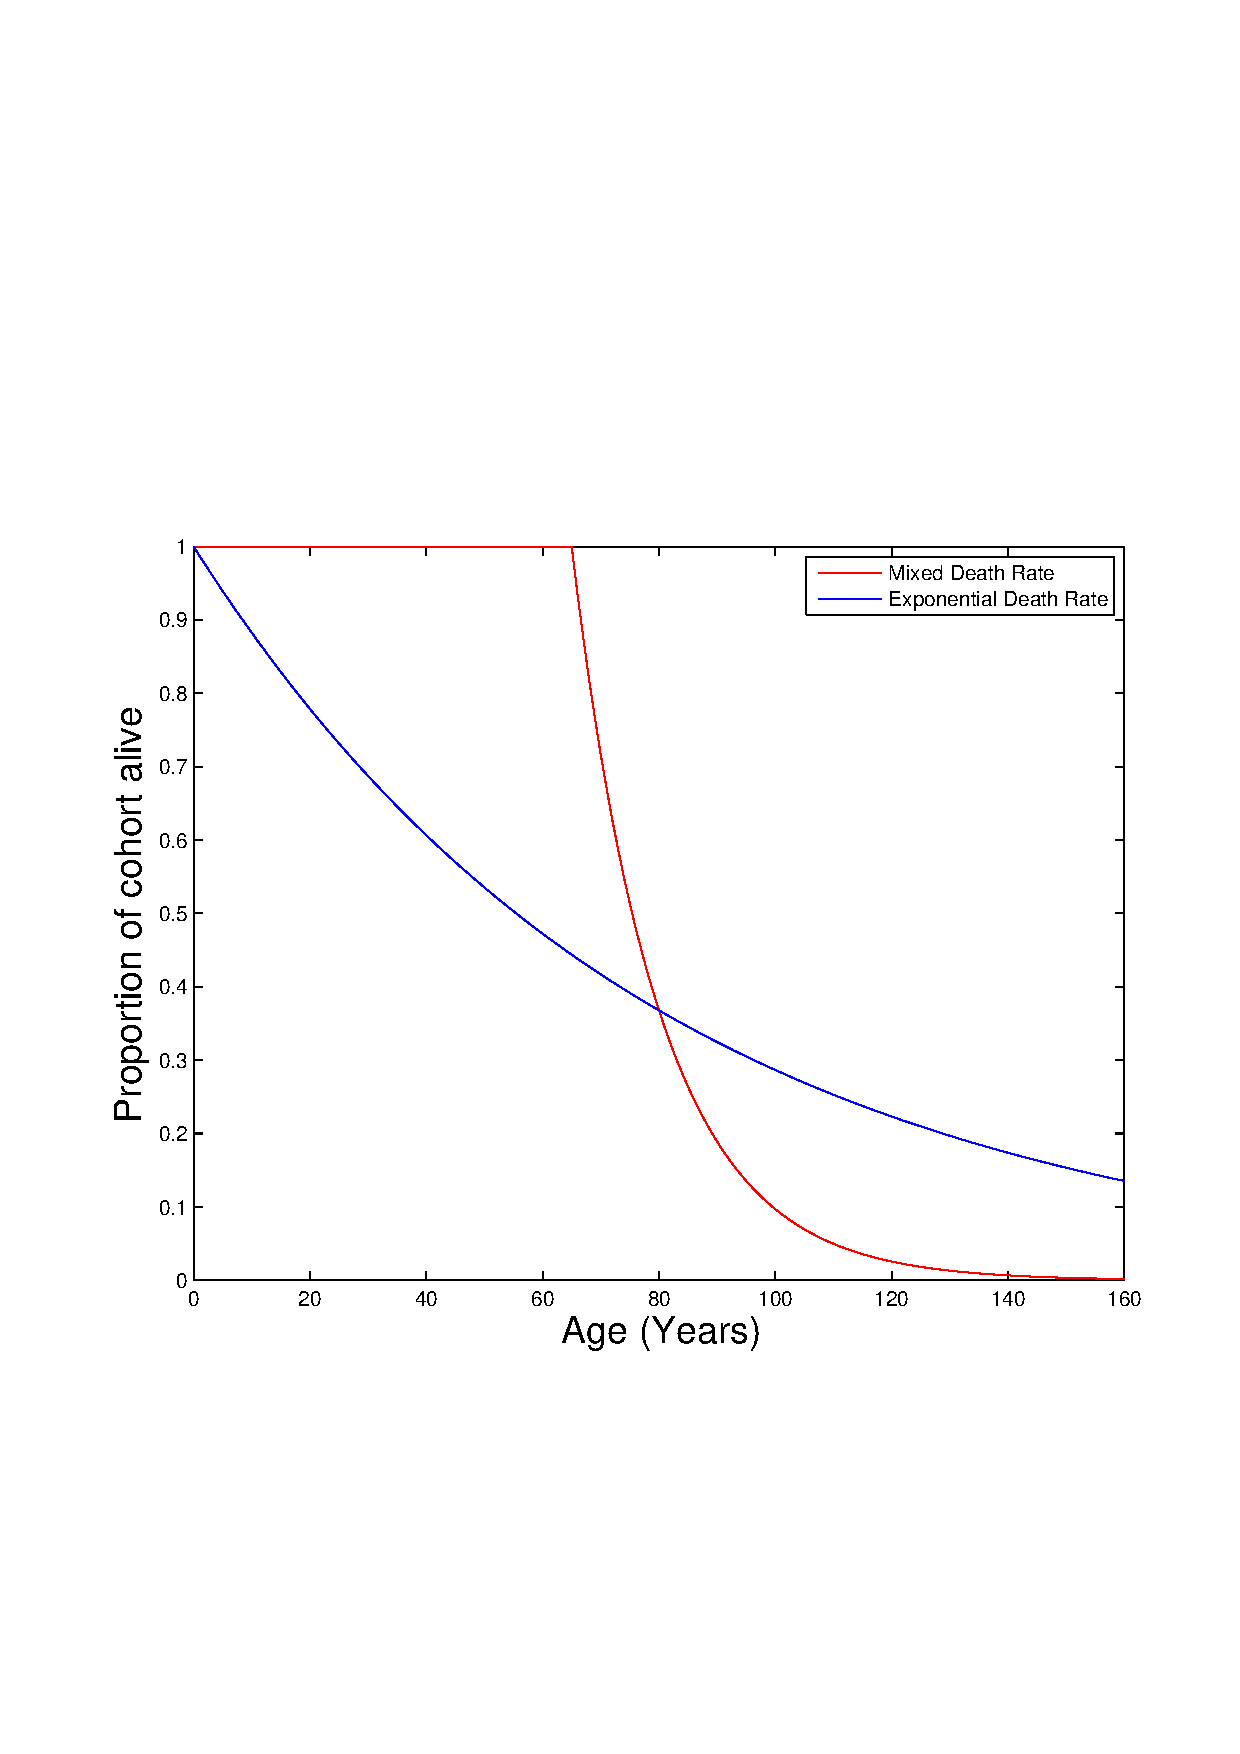
\includegraphics[width=80mm]{comparisoncumulativealive}
	\caption{Proportion of a cohort still alive as the cohort ages. A comparison of an exponentially distributed death rate against the mixed death rate $\alpha(a)$.}
	\label{fig:estimateparametersdeathcdf}
\end{figure}

The study follows Levin et al.\cite{levin2011global} in using experimentally obtained age-dependent contact rates as the basis for transmission rates. In age-structured models, transmission rates are implemented using `who acquires infection from who'\ (WAIFW) matrices\cite{anderson1985age, keeling2011modeling}. These have previously been estimated by inference from infection statistics and choice of matrix structure\cite{edmunds2000pre}. In contrast, I assume that the rate of transmission $\beta$ is dependent on the number of interactions an individual has and the transmission risk of the disease. Contact matrices give the number of interactions an individual of a given age $j$ has with individuals of age $i$ in a year. The transmission risk of each disease $\kappa$ is the probability of infection per contact.

 Mossong et al.\cite{mossong2008social} determines both physical and non-physical contact matrices in European countries. MMR is spread through droplets of moisture from the nose or throat of an infectious individual\cite{nhschoicesmeasles,nhschoicesmumps,nhschoicesrubella}. Hence, they can be spread without physical contact, so I use the UK physical and non-physical contact matrix Mossong et al.\cite{mossong2008social} as my contact matrix C (see \autoref{matrix:contactmatrix} in Appendix).

Deciding which age groups are used within the model is primarily dependent on the contact matrix data available. Accuracy shorter than one month intervals would make the computational time required too large. Intervals larger than one month would make the loss of maternal immunity data course. Consequently, I use monthly birth cohorts. These birth cohorts are tracked until all vaccinations are administered. For comparison of different vaccination schedules, the age groups must be the same in all models, hence I must track the birth cohorts until 18 years of age. As the contact matrix $C$ has 5 year age groups, the age group after 18 is 20--25 years, so I track monthly cohorts until 20 years of age hence $m=240$. After 20 years, individuals are added to the age groups with ageing parameter $\omega$. As $C$ has age groups 5 year wide I maintain this, hence $n=11$. This requires less alteration of $C$ and fewer assumptions about population interaction. Beyond 70 years, individuals are added to the 70+ age group and I no longer track their age. There are 251 age groups, those 1--240 are monthly cohorts, those 241--250 are 5 year wide cohorts and 251 is for those 70+. Consequently, $\omega(i)=1/5$, the ageing parameter, is the inverse of the age group width for $i=241,\dots,250$.

I want an easily detectable passage of time due to monthly cohorts. The simplest method is using a counter but months are irregular. However, months occur approximately every $30$ days and there are 12 months within a year. So I use the step size of $h = 1/360$, an approximate day with months occurring 30 approximate days.

Due to the introduction of monthly birth cohorts the age groups 0--5, 5--10, 10--15 and 15--20 must be sub-divided into monthly cohorts. I assume uniform contact within a 5 year age groups (e.g. the number of contacts with 7 month old individuals is the same as the number of contacts with 12 month old individuals as they are both contained within 0-5 years group). Consequently divide the contact matrix into sub-matrices. 
\begin{equation*}
C = \bordermatrix{\text{Age Group}& 0\text{--}20 & 20\text{--}70+ \cr
0\text{--}20 & Q1 & Q2\cr
20\text{--}70+ & Q3 & Q4 \cr
}
\end{equation*}
From $C$ I need to create an extended contact matrix $\hat{C}$ representing the number of contacts in a year. From Mossong et al.\cite{mossong2008social}, each column in the contact matrix $C$ represents the average number of contacts an individual from an age group has with each age group in a day. Each matrix entry $c_{i,j}$ in $Q1$ must be divided by 60, as there are 60 monthly cohorts contained within each 5 year wide group and becomes a $60 \times 60$ matrix containing entries $\frac{c_{i,j}}{60}$. Similarly each $Q2$ matrix entry $c_{i,j}$ must be divided by 60 and become a $60 \times 1$ matrix (column vector) containing entries $\frac{c_{i,j}}{60}$. Within $Q3$ each matrix entry $c_{i,j}$ remains the same and becomes a $1 \times 60$ matrix (row vector) containing $c_{i,j}$. $Q4$ is not altered. As there are 360 days in my approximate year and the contact matrix C is the number of contacts in a day, so this must be multiplied by 360 to give the a $251 \times 251$ extended contact matrix $\hat{C}$.

The transmission rate $\beta$ is assumed to be a combination of total contacts per year, given by the extended contact matrix $\hat{C}$, and the transmission risk $\kappa$ i.e. $\beta = \kappa \hat{C}$. The data available for transmission risks for each disease is limited and must be approximated. Details on the approximation of $\kappa$ can be found in \autoref{subsec:estimateparametersinitialconditions}.

\subsection{Disease parameters}
\label{subsec:estimateparametersdisease}
I assume an exponential distribution for recovery and progression, although not realistic it gives a good approximation. Recovery and progression rates are taken from Anderson and May\cite{anderson1982directly}, as a range is specified I take the mean infectious and latent periods respectively. The progression and recovery rates must be per year. So invert the mean number of days for the latent and infectious periods. Then multiply by 360, the approximate number of days per year.

\begin{table} [h]
\centering
\begin{tabular}{c c c c c}
\toprule
& & \multicolumn{3}{c}{Diseases} \ \\
\multicolumn{2}{c}{Parameter} & Measles & Mumps & Rubella \\
\midrule
Progression rate & $\sigma$ & $360/7.5$ & $360/15$ & $360/10.5$ \\
Recovery rate & $\gamma$ & $360/6.5$ & $360/6$ & $360/11.5$\\
Transmission risk & $\kappa$ & 0.11 & 0.08 & 0.02\\
\bottomrule
\end{tabular}
\caption{Disease parameters.}
\label{tab:estimateparameterdiseaseparameters}
\end{table}

\subsection{Waning of vaccine derived immunity}
\label{subsec:estimateparameterswaning}
I consider two models; one in which vaccinated immunity does not wane (i.e. $\psi_i = 0$) and one where vaccinated immunity is lost at some rate. LeBaron\cite{lebaron2007measlespersistence,lebaron2009mumpspersistence,lebaron2009rubellapersistence} and Davidkin\cite{davidkin2008persistence} follow a cohort before and after MMR2 is administered at approximately 6 years. These studies were carried out in environments in which encountering MMR was unlikely. I use data from Davidkin as the study was over a longer period of time. Davidkin\cite{davidkin2008persistence} reports 15 years after MMR2 that 95\%, 74\% and 100\% of the study population have immunity against MMR respectively.

There are very few recent studies examining loss of immunity in those receiving just one dose of MMR and due to the limited data I approximate waning immunity in those with one-dose of vaccine. I assume an exponential distribution and that the proportion maintaining vaccinated immunity 15 years after one dose is 10\% lower than the proportion maintaining vaccinated immunity 15 years after a second dose. Similarly, there is no appropriate data examining the loss of immunity in those who received three doses of MMR. Consequently, I make the somewhat drastic assumption that immunity does not wane after 3 doses of vaccination. This assumes an individual who gets 3 vaccination doses has lifelong protection, even if the first dose of vaccination failed because of maternal immunity.

Accounting for waning immunity is important for successful modelling of vaccination schedules, but accurately determining it is still problematic. It is unclear what constitutes immunity and the manner in which it is lost. Establishing immunity thresholds can be difficult and for mumps there is currently no established antibody level for protection\cite{davidkin2008persistence}. There are factors which are difficult to account for which can impact the duration of vaccinated immunity such as natural antibody boosting and the age at which vaccination is administered.

\begin{table} [h]
\centering
\begin{tabular}{c c c c c c c c}
\toprule
& \multicolumn{2}{c}{15 years post vaccine(\%)} 
& \multicolumn{2}{c}{30 years post vaccine(\%)} &&&\\
Disease& 1st dose 
& 2nd dose\cite{davidkin2008persistence}& 1st dose 
& 2nd dose& $\psi_1$ & $\psi_2$ & $\psi_3$\\
\midrule
Measles &85 & 95 & 72.3 & 90.3 & 1.08\powers{10}{-2} & 3.42\powers{10}{-3} & 0\\
Mumps &64 & 74 & 41 & 54.8 & 2.98\powers{10}{-3} & 2.01\powers{10}{-3}& 0\\
Rubella & 90 & 100 & 81 & 100 & 3.42\powers{10}{-3} & 0 & 0\\
\bottomrule
\end{tabular}
\caption{Parameters for the waning of vaccine derived immunity. The percentage still immune after a period of time for those whom vaccine was successful.}
\label{tab:estimatewaningimmunity}
\end{table}

\subsection{Cost of infection and vaccination}
\label{subsec:estimateparameterscost}
Carabin et al.\cite{carabin2003cost} outline the cost of MMR vaccination in various European countries, I use UK data. Delivery of MMR is US\$13.4(2001) and the MMR vaccine is \$8.7. The cost of the adverse effects of vaccination is given by Carabin et al.\cite{carabin2002average} at \$1.93. Hence, total cost of vaccination is \$24.03.

Up to date European data on cost of infection is limited to measles\cite{carabin2002average,beutels2002difficult}. I use the UK figures from Carabin et al.\cite{carabin2002average}, who give the cost of a case of measles as \$307. Due to the limited data I estimate the cost of a mumps, rubella and CRS using other cost analyses. I obtained three such studies: Hinman(USA, 2004)\cite{hinman2004economic}, White(USA, 1985)\cite{white1985benefits} and Pelletier(Canada, 1998)\cite{pelletier1998benefit}. I use Pelletier\cite{pelletier1998benefit} as it clearly outlines the total cost per case. I calculate the ratio per case to per case of measles and multiply this ratio by the cost of measles from Carabin et al.\cite{carabin2002average}. This is a rather rough approximation of the underlying costs associated with mumps, rubella and CRS and highlights the sparsity of data currently available concerning cost in the UK of these disease.

\begin{table} [h]
\centering
\begin{tabular}{c c c c}
\toprule
Item & Cost per case (Pelleltier\cite{pelletier1998benefit}) & Measles:Item Ratio & Cost per case(US\$ 2001)\\
\midrule
Vaccination & - & - & \textbf{24}\\
Measles & 929 & N/A & \textbf{307}\\
Mumps & 390 & 0.42 & \textbf{129}\\
Rubella & 394 & 0.42 & \textbf{130}\\
CRS & 514853 & 163.87 & \textbf{170140}\\ 
\bottomrule
\end{tabular}
\caption{Cost per case of MMR and CRS rounded to the nearest \$.}
\label{tab:estimateparametercosts}
\end{table}

\subsection{Initial conditions}
\label{subsec:estimateparametersinitialconditions}
First I estimated the stable age distribution by running the model containing only susceptible individuals for 200 years. This estimated stable age distribution can be found in \autoref{tab:estimatewaningstableagedistribution}. Within the model the initial conditions are at the beginning of a month. We assume that group 1 has population of 0 in the stable age distribution, as newborns enter group 1 at each time step but this is reset to 0 at the start of every month with the occurrence of discrete events.

\begin{table} [h]
\centering
\begin{tabular}{c c c c}
\toprule
Age Group(s) & Age Bound & \# & Total\\
\midrule
1 & 0-1 months & 0 & 0\\
2-240 & 1-240 months & 65,680 & 15,697,520 \\
241-249 & 20-65 years & 3,942,525 & 35,482,725\\
250 & 65-70 years & 2,953,250 & 2,953,250\\
251 & 70+ & 8,866,505 & 8,866,505\\
\bottomrule
\end{tabular}
\caption{Stable age distribution.}
\label{tab:estimatewaningstableagedistribution}
\end{table}

$\kappa$ was then established for each disease. Two important factors to consider were the average age of infection and temporal occurrence of epidemics, a summary can be found in \autoref{tab:estimatediseaseattributes}. The number of infectious individuals was set to 25,000, susceptibles ($S_0$) set to 3,000,000 with the remaining 59,975,000 in the recovered group. The same age distribution as in \autoref{tab:estimatewaningstableagedistribution} was used with the proportion within each state uniform across each age group. Call this the temporary start distribution. The model using the temporary start distribution for various $\kappa$ was run for 100 years. The occurrence of epidemics after 30 years was then analysed and the average age of infection between years 70 and 100 was determined. $\kappa$ is chosen to best satisfy observed results in \autoref{tab:estimatediseaseattributes}. The average age of infection for various $\kappa$ is in \autoref{tab:kappacomparison} in the Appendix. Unfortunately Levin et al.\cite{levin2011global} which uses the same method for determining transmission rate $\beta$ does not detail the $\kappa$ value used. This trial and error approach is not ideal and further research must be carried out for more rigorous approximations of transmission risk to take advantage of contact matrices in Mossong et al.\cite{mossong2008social}. 

\begin{table} [h]
\centering
\begin{tabular}{c c c}
\toprule
Disease & Interepidemic period (Years)\cite{anderson1985age} & Average age of infection (Years)\\
\midrule
Measles & 2--3 & 4.44--5\\
Mumps & 3--4 & 5.71--7.27\\
Rubella & 3--5 & 11.4--13.3\\
\bottomrule
\end{tabular}
\caption{Disease attributes. The average age of infection calculated using $\frac{L}{R_0}$. $L=80$, the life expectancy in the model. $R_0$ data taken from England and Wales in Anderson and May\cite{anderson1991infectioustable}.}
\label{tab:estimatediseaseattributes}
\end{table}

Once $\kappa$ was established, the stable age distribution with infection could be determined. The temporary start distribution was used and the model was run for 200 years to estimate the stable age distribution with infection. When compared with the stable age distribution without infection, the two were extremely similar. Hence, the start distribution is the temporary start distribution.

Disease specific initial conditions are determined. For all diseases the model is run for 50 years without vaccination using the start distribution. Vaccination performed in the UK is replicated for each disease, detailed coverage information can be found in \autoref{tab:vaccinationcoverage} in the Appendix. Vaccination is then introduced into the model. For measles only, 20 years of a single dose of vaccine at 12 months with 55\% coverage is performed simulating vaccination before the introduction of MMR. Then for all diseases, to simulate MMR vaccination, a single dose of vaccine at 12 months with 85\% coverage is administered for 10 years. This is followed by a double dose vaccination scheme where first dose is at 12 months and second dose is at 5 years with 85\% coverage. This gives initial conditions for the model without waning and with waning.

\subsection{Discussion}
\label{subsec:estimateparametersdiscussion}
This chapter is better thought of as a shopping list for parameters. Many of these are yet to be properly estimated, and my parameter estimation highlights where further research is required. I believe further research into waning of vaccinated immunity is required, as it is likely to impact on long term successes of vaccination schedules. Up to date cost estimation for mumps, rubella and CRS are required for a detailed cost analysis of the MMR vaccine in the UK. The risk of transmission per contact is difficult to study, predominately because there are ethical issues of allowing individuals to become infected. Once good estimates of the transmission risks have been determined, this will allow excellent estimates of transmission rates. That said, this does not account for all forms of transmission as infection can be transmitted via formites on shared surfaces, a type of contact not captured in the Mossong data. Ultimately, if similar analyses to this study were to be performed by decision makers, resources must be allocated for accurate estimation of many of these parameters.

\newpage
\section{Results}
\label{sec:results}
For brevity, results are only presented for measles. Parameters have been established for both mumps and rubella so it would be simple to run the model with these parameters. The model is run for 50 years and the results are analysed to answer the following questions. Will current vaccination coverage eliminate measles in the UK? How will the age profile of susceptibility in infants change as a result of changes to immunity in mothers? Does this necessitate a change in the age at which MMR1 is administered? What would occur if vaccination coverage of 95\% were achieved\footnote{This is in line with vaccination coverage attained for most recommended vaccinations\cite{hpaimmunistationcoverage}}? Is a single dose of vaccination justified? How will vaccination alter the occurrence of infection? How does the total cost of vaccination schedules change as vaccination coverage is changed?

Under waning immunity we ask further questions of the model. How many individuals that have received vaccination become infected? Can a triple dose of vaccination be recommended?

\subsection{Comparison of initial conditions to reality}
\label{subsec:resultscomparison}
The behaviour of the model in the 50 years prior vaccination can be seen in \autoref{fig:resultsmeaslesprevaccinaiton}. After 35 years, the model begins to approach equilibrium. Epidemics occur approximately every 2.5 years, in comparison to 2--3 years observed in reality. In epidemic year 41 and non-epidemic year 42 there were 1,150,000 and 580,000 new infections respectively. Notified cases in England and Wales prior vaccination were 6--700,000 in epidemics years and 3--400,000 in non-epidemic years (see \autoref{mmrnotifications1989} in Appendix). These modelled results compare well with reality, considering the population of England and Wales in the 1951 and 1961 was 43,000,000 and 46,000,000 respectively\cite{census1951,census1961} and the population within the model is 63,000,000. The force of infection at the end of this 50 year period can be found in \autoref{fig:estimateparametersforceofinfection}.
\begin{figure}[h]
	\centering
	\includegraphics[width=80mm]{measlesprevaccination}
	\caption{The number of susceptible individuals and new infections at each time step. The 50 years that the model is run prior the introduction of vaccination.}
	\label{fig:resultsmeaslesprevaccinaiton}
\end{figure}

However, post-vaccination the number of new infections within the model is larger than the notified cases (see \autoref{tab:priorinitialisationcomparison} in the Appendix). In particular, when coverage was low, the difference between the model without waning and the notified cases is large. There are variety of possible reasons. The model has a population of 63,000,000 (UK current) but the notified cases are from England and Wales and the population has increased since the initial data was collected. However, this could only explain a small discrepancy. Contact rates may change over time as population density increases or other social factors change, such as family size. This seems unlikely, as the same contact matrices correspond well with infection before vaccination. Under-reporting of cases of measles in historical data is possible. This too seems unlikely to be the major cause, as the modelled results are similar to the notified cases before vaccination. Spatial homogeneity could be a factor. Coverage is assumed to be uniform and mixing is not location dependent. Within the model, epidemics occur throughout the entire population and can infect high numbers of people. With varying regional coverage and mixing, epidemics may occur in some regions and a not in others due high coverage or infection may effect some regions more severely than others. Further investigation on the impact of spatial homogeneity is required to understand its impact on the number of infections.
\begin{figure}[h]
	\centering
	\includegraphics[width=90mm]{forceofinfectioncomparison}
	\caption{Force of infection for measles. No vaccination is the model after it has been run for 50 years without vaccination. Initial is the initial distribution after the replication of vaccination.}
	\label{fig:estimateparametersforceofinfection}
\end{figure}

\subsection{Without waning of vaccine derived immunity}
\label{subsec:resultsnowaning}
Without waning  of vaccine derived immunity, MMR3 cannot bestow any additional immunity as MMR2 is administered after all protective maternal immunity has been lost. Those who received MMR2 have vaccinated immunity which will not wane, so the only difference between double and triple vaccination is the cost of the additional dose of vaccine. Hence, triple vaccination will not be examined.

The behaviour of the model if the current vaccination schedule is maintained with 85\% coverage is given by \autoref{fig:resultsmeaslesnowaningdouble85}. Epidemics occur approximately every 12 years. In the non-epidemic year 30, there are 4,619 new infections. In the epidemic year 35 there are 271,400 new infections. An average of 72,000 new infections per year occur over the 50 year period. An age-distributed break down of infections is given in \autoref{fig:resultsyearlytotalinfectionsdouble85}. 

\begin{figure}[hp]
	\centering
	\includegraphics[width=100mm]{measlesnowaningdouble85}
	\caption{The number of susceptible individuals and new infections at each time step within the model. The model is run for a period of 50 years. The first dose of vaccine is at 12 months and second dose is at 5 years. Vaccination coverage is 85\%.}
	\label{fig:resultsmeaslesnowaningdouble85}
	
	\includegraphics[width=120mm]{yearlytotalinfectionsdouble85}
	\caption{The total number of new infections occurring within each age group each year that the model is run. The model is run for a period of 50 years. The first dose of vaccine is at 12 months and second dose is at 5 years. Vaccination coverage is 85\%.}
	\label{fig:resultsyearlytotalinfectionsdouble85}
\end{figure}

\begin{figure}[hp]
	\centering
	\includegraphics[width=100mm]{maternalimmunitymeaslesnowaningdouble85}
	\caption{The proportion of the infant population with protective maternal immunity (either in $M_V$ or $M_R$). No vaccination is after the model has run for 50 years without vaccination. Initial is at the initial conditions. After 30 years is 30 years after the initial conditions. The first dose of vaccine is at 12 months and second dose is at 5 years. Vaccination coverage is 85\%.}
	\label{fig:resultsmaternalimmunitymeaslesnowaningdouble85}
	
	\includegraphics[width=100mm]{infectionininfantsnowanedouble85}
	\caption{The number of infants infected during an epidemic year. No vaccination is an epidemic after the model has run for approximately 50 years without vaccination. Initial is year 0 after initial conditions, the first epidemic after the initial conditions. After 30 years is epidemic year 35 after initial conditions, the first epidemic after 30 years. The first dose of vaccine is at 12 months and second dose is at 5 years. Vaccination coverage is 85\%.}
	\label{fig:resultsinfectionininfantsnowanedouble85}
\end{figure}

The number of infections occurring within the model seems much higher during epidemics than has been observed since high coverage of measles vaccine has been attained (see \autoref{tab:priorinitialisationcomparison}). Some possible reasons have been suggested in \autoref{subsec:resultscomparison}. However, we may not have yet seen a severe epidemic of measles in the high coverage era. Coverage $>80\%$ has been maintained since 1988/9 and the last severe epidemic of measles was in 1988 with 86,001 notified cases. The model suggests that epidemics occur approximately every 12 years at 85\% coverage and coverage $>85\%$ throughout the 1990s could have increased the period between epidemics. A severe epidemic of measles in the near future could be possible if coverage remained low.

Alternatively, unrealistic extended contact matrix assumptions in infants could be a factor. It is unlikely a 4 year old has the same contacts as an infant. The infant group (0--1 years) are highly susceptible, during epidemics high numbers of infants become infectious. \autoref{fig:resultsyearlytotalinfectionsdouble85} shows the infant group (0--1) has more infections during epidemics than the 1-5 years group despite being a quarter of the size. Whereas, 2012 UK data\cite{hpameasles2012cases} showed there were 376 infections in those aged 1--5 years in comparison to 216 in those aged 0--1 years. Consequently, within the model, infants may help spread infection and increase the number of infections. This suggests more detailed contact matrices may be needed for infants and toddlers when accounting for maternal antibodies. Numerical experimentation showed removing contacts with infants reduced infections during an epidemic, but could not explain the significant increase.

\autoref{fig:resultsmaternalimmunitymeaslesnowaningdouble85} shows the past, present and future of the proportion of infants with protective maternal immunity. Before vaccination was introduced, the proportion of infants with maternal immunity is almost identical to Figure\autoref{fig:establishingparametersmeaslesrec}. This is because the vast majority of those of childbearing age are in the recovered group. The model shows a substantial decline of infants with protective maternal immunity since the introduction of vaccination, as a high proportion of the childbearing population have vaccine derived immunity. As high coverage is maintained over the next 30 years, the population of infants with maternal immunity decreases further. The longer high coverage is maintained, the higher the proportion of the childbearing population with vaccine derived immunity (up to 85\%). The proportion of mothers recovered from measles decreases and those susceptible increases.

\autoref{fig:resultsinfectionininfantsnowanedouble85} shows the number of infections occurring within the infant population during epidemic years. Infections in the infant group before vaccination is approximately 120,000 with 72.4\% of those occurring in those aged 6 months or over. Whereas the number of infections occurring near initial conditions and after 30 years are both approximately 23,500, with 65\% and 62.7\% occurring in those aged 6 months or over respectively. This suggests as high vaccination coverage is maintained, the proportion of measles cases within very young infants increases. However, this is based on the uniform contact assumption of the extended contact matrix which may not be realistic.

If coverage is increased to 95\%, the behaviour is shown in \autoref{fig:resultsmeaslesnowaningdouble95}. Elimination is achieved after year 5 and the number of susceptible individuals increases as infection no longer occurs. After year 30 the number of susceptibles decreases. Post-elimination, the only two ways in which of the number of susceptibles can decrease is either via vaccination or death. If the system was run for an infinite amount of time the number of susceptible individuals would be the proportion of the population not vaccinated (i.e. 5\% of 63 million 3,150,000). Hence, the number of susceptible individuals will tend towards this number. Examining the age distribution of susceptible individuals in \autoref{fig:resultssusceptibles3double95}, we see the high number of susceptible individuals in the 5--30 age group initially. This high number of susceptible individuals then propagates through the age groups as time progresses and the population ages, reaching the oldest age groups where death occurs.

\begin{figure}[hp]
	\centering
	\includegraphics[width=100mm]{measlesnowaningdouble95}
	\caption{The number of susceptible individuals and new infections at each time step within the model. The model is run for a period of 50 years. The first dose of vaccine is at 12 months and second dose is at 5 years. Vaccination coverage is 95\%.}
	\label{fig:resultsmeaslesnowaningdouble95}

	\includegraphics[width=120mm]{susceptibles3double95}
	\caption{The number of susceptible individuals within each age group at each year the model is run. The model is run for a period of 50 years. The first dose of vaccine is at 12 months and second dose is at 5 years. Vaccination coverage is 95\%.}
	\label{fig:resultssusceptibles3double95}
\end{figure}

Due to the lack of waning immunity and the parameters used for maternal immunity, single dose vaccination schemes have very similar behaviour to double vaccination schemes. Consequently, I do not include a detailed analysis for single dose vaccination.

The results presented have a higher number of infections than would be expected from data on measles cases in England and Wales\cite{hpameaslesnotificationsanddeaths}. The reason is not clear and numerous possibilities have been suggested. Consequently, estimates of the cost of infection may be higher than reality. A breakdown of the cost of the current vaccination schedule is shown in \autoref{fig:resultscostnowaningcurrent}. At 85\% coverage the total cost of the current vaccination schedule is US\$2.713bn (2001) over the next 50 years with \$1.110bn attributable to the costs of measles cases. Elimination is achieved at 89\% coverage. These results show that it is more cost effective to overvaccinate than undervaccinate a population. The wobbles in the cost of infection correspond to epidemics. Each wobble represents to one fewer epidemic occurring during 50 year period as coverage increases. Aiming for a coverage of 95\% is sensible, as there is an estimated \$810m saving over 50 years  and successful elimination of measles from the UK when compared to coverage of 85\%.

A comparison of the total cost of different vaccination schedules is given in \autoref{fig:resultscostnowaningcomparison}. Elimination is achieved at 89\% for all double dose vaccination schedules and 90\% for all single dose schedules. Differences between cost of single dose vaccination schedules at coverage rates above this is are due to infections before elimination. Single dose vaccination schedules are more cost effective than double dose vaccination schedules at the same coverage. With coverage at 95\%, if MMR2 was dropped and MMR1 continued to be administered at 12 months then \$890m could be saved over 50 years. Of the single dose schemes, vaccination at 9 months has the greatest total cost, between 75--92\% coverage it costs in excess of \$100m more than vaccination at 11 and 12 months. At high coverage there is not much difference between vaccinating at 10,11 or 12 months as the lowest total cost between 80--90\% coverage is not clear. Comparing the double dose vaccination schedules, there is little distinction between them. With coverage below 80\% the total cost of all the double dose vaccination schedules are almost identical. With coverage between 80--89\% no schedule clearly offers the lowest total cost.

\begin{figure}[hp]
	\centering
	\includegraphics[width=120mm]{costnowaningcurrent}
	\caption{The cost of the current vaccination schedule varying vaccination coverage. First dose is at 12 months and second dose is at 5 years. No waning of vaccine derived immunity.}
	\label{fig:resultscostnowaningcurrent}

	\includegraphics[width=120mm]{costnowaningcomparison}
	\caption{Comparison of the total cost of vaccination schemes varying vaccination coverage. Dashed lines are single dose vaccination schemes and solid lines are double dose vaccination schemes. No waning of vaccine derived immunity.}
	\label{fig:resultscostnowaningcomparison}
\end{figure}

\newpage
\subsection{Including waning of vaccine derived immunity}
\label{subsec:resultswaning}
The behaviour of the model maintaining current vaccination is given by \autoref{fig:resultsmeasleswaningdouble85}. Epidemics occur approximately every 7.5 years, in comparison to every 12 years without waning. The number of infections is higher too, with approximately 94,000 and 305,000 new infections occurring in non-epidemic year 30 and epidemic year 34 respectively. Over the 50 year period, there is an average of 190,000 infections annually. This this is very many more than the observed results of 2--3,000 notified infections in non-epidemic years and 5,000 notified infections in `epidemic'\ years since vaccination (see \autoref{mmrnotifications}).

\begin{figure}[h]
	\centering
	\includegraphics[width=100mm]{measleswaningdouble85}
	\caption{The number of susceptible individuals and new infections at each time step within the model. The model is run for a period of 50 years. The first dose of vaccine is at 12 months and second dose is at 5 years. Vaccination coverage is 85\%. Waning of vaccine derived immunity is included.}
	\label{fig:resultsmeasleswaningdouble85}
\end{figure}

A breakdown of infections by age and the number of doses of vaccine received is given in \autoref{fig:resultsinfectiondosesbreakdowndouble85}. Double vaccination was introduced 15 years before the initial conditions. Consequently, no individuals aged 5--20 become infected after one dose of vaccine. In total, 2,100,000 individuals infected after one dose of vaccine were 20+. These are those individuals vaccinated during the era of single dose vaccination. It may therefore be beneficial to offer a catch-up programme for those who only received a single dose of vaccination. 75,600 individuals in the 1--5 age group became infected after one dose, in between their first and second dose of vaccine. There were approximately 1,700,000 individuals infected having received 2 doses of vaccine, 17.8\% of infections.

\begin{figure}[h]
	\centering
	\includegraphics[width=100mm]{infectiondosesbreakdowndouble85}
	\caption{The number of infections occurring over the 50 year period. The data is broken down into age group and the number of doses of vaccine received when exposed. The first dose of vaccine is at 12 months and second dose is at 5 years. Vaccination coverage is 85\%.}
	\label{fig:resultsinfectiondosesbreakdowndouble85}
\end{figure}

The impact of increasing vaccination coverage to 95\% is given in \autoref{fig:resultsmeasleswaningdouble95}. Epidemics occur approximately every 15 years. In contrast to the model without waning, measles is not eliminated. In epidemic year 35 there were 63,000 new infections and in the non-epidemic year 30 there were 46,000 new infections. In the USA, coverage of $>90\%$ has been maintained since 1996 and measles was eliminated in 2000\cite{cdcmeasleselimination}. This indicates that the assumed exponential decay of vaccinated immunity is likely to be inaccurate. The modelled average number of infections annually is 64,000. 

\autoref{fig:resultsmeasleswaningsingle95} shows what occurs if MMR2 is dropped with coverage of 95\%. Epidemics occur approximately every 6 years. The number of new infections in epidemic year 23 is approximately 390,000 and 159,000 in non-epidemic year 25. An average over the 50 year period is 254,000 new infections annually. These figures are significantly higher expected and higher than the number of infections that occurred in the England and Wales at significantly lower vaccination coverage (see \autoref{tab:priorinitialisationcomparison}).

\begin{figure}[hp]
	\centering
	\includegraphics[width=100mm]{measleswaningdouble95}
	\caption{The number of susceptible individuals and new infections at each time step within the model. The model is run for a period of 50 years. The first dose of vaccine is at 12 months and second dose is at 5 years. Vaccination coverage is 95\%. Waning of vaccine derived immunity is included.}
	\label{fig:resultsmeasleswaningdouble95}

	\includegraphics[width=100mm]{measleswaningsingle95}
	\caption{The number of susceptible individuals and new infections at each time step within the model. The model is run for a period of 50 years. The first dose of vaccine is at 12 months. Vaccination coverage is 95\%. Waning of vaccine derived immunity is included.}
	\label{fig:resultsmeasleswaningsingle95}
\end{figure}

Both \autoref{fig:resultsmeasleswaningdouble95} and \autoref{fig:resultsmeasleswaningsingle95} demonstrate the impact of including waning immunity, showing vaccination schedules which would eliminate measles if vaccine induced immunity endures no longer achieve elimination. The main result of the model when vaccine induced immunity wanes is that the results are incompatible with the past 20 years of measles epidemiology. This highlights the importance of acquiring an improved understanding of the duration of vaccine induced immunity.

\autoref{fig:resultsmeasleswaningtriple95} shows the impact of introducing a third dose of vaccine at 18 years with coverage at 95\%. Elimination is achieved at year 20. This is most likely because immunity is assumed to be lifelong after MMR3. \autoref{fig:resultsmeasleswaningtriple95} shows similar behaviour to \autoref{fig:resultsmeaslesnowaningdouble95}. The number of susceptible individuals rises to over 7,000,000 at year 33 before declining. As before, post-elimination the number of susceptible individuals tends towards the proportion of the population not vaccinated.

\begin{figure}[h]
	\centering
	\includegraphics[width=100mm]{measleswaningtriple95}
	\caption{The number of susceptible individuals and new infections at each time step within the model. The model is run for a period of 50 years. The first dose of vaccine is at 12 months, the second dose is at 5 years and third dose is at 18 years. Vaccination coverage is 95\%. Waning of vaccine derived immunity is included and the third dose of vaccine is assumed to bestow lifelong immunity.}
	\label{fig:resultsmeasleswaningtriple95}
\end{figure}

The cost of the current vaccination can be found in \autoref{fig:resultscostmeasleswaningdoublecurrent}. With the inclusion of waning, the model shows elimination will not be achieved, even with 100\% coverage there is a \$270m cost of infection. \autoref{fig:resultscostmeasleswaningdoublecurrent} shows, like \autoref{fig:resultscostnowaningcomparison}, it is more cost effective to overvaccinate than undervaccinate a population. At 85\% coverage, total cost is \$4.515bn and cost of infection is \$2.924bn. Comparing \autoref{fig:resultscostmeasleswaningdoublecurrent} with \autoref{fig:resultscostnowaningcurrent}, the cost of infection with waning is almost 3 times the cost of infection without waning. If coverage was increased to 95\%, total cost is \$2.769bn with \$985m associated with infection, showing a large decrease in total cost and the number of infections. At low coverage, the cost of infection with and without waning immunity is similar. However, at high coverage there is a greater difference between the cost of infection with and without waning immunity.

\begin{figure}[hp]
	\centering
	\includegraphics[width=120mm]{costmeasleswaningdoublecurrent}
	\caption{The cost of the current vaccination schedule varying vaccination coverage. First dose is at 12 months and second dose is at 5 years. Waning of vaccine derived immunity is included.}
	\label{fig:resultscostmeasleswaningdoublecurrent}
\end{figure}
\begin{figure}[hp]
	\centering
	\includegraphics[width=120mm]{costmeasleswaningdouble}
	\caption{Comparison of the total cost of double vaccination schedules varying vaccination coverage. The legend shows when the first dose of vaccine is administered. The second dose of vaccine is at 5 years. Waning of vaccine derived immunity is included.}
	\label{fig:resultscostmeasleswaningdouble}
\end{figure}

A comparison double and triple dose vaccination schedules can be found in \autoref{fig:resultscostmeasleswaningdouble} and \autoref{fig:resultscostmeasleswaningtriple} respectively. There is no substantial difference in total cost between the double vaccination schedules. Similarly for the triple vaccination schedules. 
\begin{figure}[h]
	\centering
	\includegraphics[width=120mm]{costmeasleswaningtriple}
	\caption{Comparison of the total cost of triple vaccination schedules varying vaccination coverage. The legend shows when the first dose of vaccine is administered. The second dose of vaccine is at 5 years and the third dose is at 18 years. Waning of vaccine derived immunity is included.}
	\label{fig:resultscostmeasleswaningtriple}
\end{figure}

The comparison of single, double and triple vaccination schemes is found in \autoref{fig:costmeasleswaningsingledoubletriple}. I include the schemes which have the initial dose of vaccine at 12 months. Single dose vaccination schedules are more costly than double and triple dose schemes due to the increased number of infections. However, this could be an artefact of the model overestimating the number of infections. With coverage below 94\% triple vaccination offers the lowest total cost, possibly driven by a larger than expected number of infections occurring under double vaccination. Elimination is achieved with triple vaccination schedules at 90\%, marginally higher than 89\% for double vaccination without waning. This is due to more susceptibles within the population in between doses of vaccination, caused by waning immunity. These results suggests, triple vaccination could be more cost effective than double vaccination when the cost of infection for mumps and rubella are included. However, this depends largely upon the waning of vaccine derived immunity which is yet to be accurately estimated.
\begin{figure}[h]
	\centering
	\includegraphics[width=120mm]{costmeasleswaningsingledoubletriple}
	\caption{Comparison of the total cost of single, double and triple vaccination schemes varying vaccination coverage. Initial dose is at 12 months for all vaccination schedules. The second dose of vaccine is applied at 5 year for double and triple. The third dose is applied at 18 years. Waning of vaccine derived immunity is included.}
	\label{fig:costmeasleswaningsingledoubletriple}
\end{figure}

\section{Conclusion}
\label{sec:conclusion}
A model has been presented that demonstrates good flexibility for analysing a variety of vaccination schedules. The model is capable of determining many factors that should be considered when deciding which vaccination schedule should be administered (e.g. the number of infected individuals having received vaccination and the impact of vaccination of different age groups). Decision makers can determine the aims of vaccination and use a model similar to the one presented in this study to determine which schemes best meet these aims. A limited range of vaccination schedules have been compared and results for measles have been presented. For a full evaluation of the MMR vaccine, similar results must be determined for mumps and rubella and a more detailed analysis performed.

The cost results of all vaccination schedules examined have shown that it is more cost effective to overvaccinate than undervaccinate a population. This a win-win situation for the health care provider and for the population, with the health care provider reducing cost and reducing the number of infections. This could justify resources being spent to increase coverage of the MMR vaccine (e.g. advertising) from 89\% (2011) to 95\% in line with other vaccinations\cite{hpaimmunistationcoverage}. There have been recent signs for optimism, UK coverage in 2011/12 was 91.6\%\cite{vaccinationcoverage2012}. However, significant work is required to restore confidence in low coverage regions (e.g. London had 86.1\% coverage in 2011/12\cite{vaccinationcoverage2012}) and communities.

Mossong et al.\cite{mossong2008social} is exciting as it paves the way for studying infectious diseases dynamics with increasing accuracy. The model captured disease dynamics and age distribution prior to vaccination well. For all 3 diseases, it gave inter-epidemic periods and average age of infection that matched historical data, despite transmission risk being determined by trial and error. This study shows further research must be carried out, in particular more detailed contact matrices amongst very young people are needed and risk of transmission should be explored further.

This study has had issues of overestimation of the number of infections, which needs to be addressed before recommending changes to vaccination schedules. In the model without waning, the number of infections seemed to be too high during epidemics. However, non-eradicating vaccination coverage rates for measles have occurred over the past decade (see \autoref{tab:vaccinationcoverage}). This has disturbing potential for large outbreaks of measles in the United Kingdom - as have been seen in Europe in 2011\cite{measleseuropeoutbreak2011}.

Results in \autoref{subsec:resultsnowaning} and \autoref{subsec:resultswaning} have shown how radically differently systems behave with and without waning immunity. This highlights that there is a lot of research still required to establish realistic rates of waning, but it is vital to a better understanding the impact of vaccination schedules.

\section*{Acknowledgements}
\addcontentsline{toc}{section}{Acknowledgements}
First and foremost I want to thank Angela McLean for being an fantastic supervisor, offering support, recommending excellent reading and for proofreading. Additionally, I want to thank everyone for tolerating me talking about nothing other than this dissertation for the last few months.

%Here are the references
\newpage
\singlespacing
\phantomsection
\addcontentsline{toc}{section}{References}
\bibliography{references}
\bibliographystyle{plain}
%end of References

\newpage
\singlespacing
\section*{Appendix} 
\label{sec:appendix}
\addcontentsline{toc}{section}{Appendix}

\begin{figure}[h]
\centering
\subfloat [Measles (Vaccinated Mothers)] {\label{fig:establishingparametersmeaslesvacc} \includegraphics[width=70mm]{measlesvacmaternal}}
\subfloat [Measles (Recovered Mothers)] {\label{fig:establishingparametersmeaslesrec} \includegraphics[width=70mm]{measlesrecmaternal}}\\
\subfloat [Mumps] {\label{fig:establishingparametersmumps} \includegraphics[width=70mm]{mumpsmaternal}}
\subfloat [Rubella] {\label{fig:establishingparametersrubella} \includegraphics[width=70mm]{rubellamaternal}}
\caption{Proportion of infants with protective maternal immunity against specified diseases. Best fit is the linear binomial regression fitted to data from Leuridan et al.\cite{leuridan2010early,leuridan2011kinetics,leuridan2012maternal}.}
\label{fig:establishingparametersmaternalimmunity}
\end{figure}

\begin{figure} [h]
\centering
C = \scalemath{0.75}{
\bordermatrix{\text{Age Group}& $0-5$ & $5-10$ & $10-15$ & $15-20$ &$20-25$ & $25-30$ & $30-35$ & $35-40$ & $40-45$ & $45-50$ & $50-55$ & $55-60$ & $60-65$ & $65-70$ & $70+$ \cr
$0-5$ & 1.92 & 0.65 & 0.41 & 0.24 & 0.46 & 0.73 & 0.67 & 0.83 & 0.24 & 0.22 & 0.36 & 0.2 & 0.2 & 0.26 & 0.13 \cr
$5-10$ & 0.95 & 6.64 & 1.09 & 0.73 & 0.61 & 0.75 & 0.95 & 1.39 & 0.9 & 0.16 & 0.3 & 0.22 & 0.5 & 0.48 & 0.2 \cr
$10-15$ & 0.48 & 1.31 & 6.85 & 1.52 & 0.27 & 0.31 & 0.48 & 0.76 & 1 & 0.69 & 0.32 & 0.44 & 0.27 & 0.41 & 0.33 \cr
$15-20$ & 0.33 & 0.34 & 1.03 & 6.71 & 1.58 & 0.73 & 0.42 & 0.56 & 0.85 & 1.16 & 0.7 & 0.3 & 0.2 & 0.48 & 0.63 \cr
$20-25$ & 0.45 & 0.3 & 0.22 & 0.93 & 2.59 & 1.49 & 0.75 & 0.63 & 0.77 & 0.87 & 0.88 & 0.61 & 0.53 & 0.37 & 0.33 \cr
$25-30$ & 0.79 & 0.66 & 0.44 & 0.74 & 1.29 & 1.83 & 0.97 & 0.71 & 0.74 & 0.85 & 0.88 & 0.87 & 0.67 & 0.74 & 0.33 \cr
$30-35$ & 0.97 & 1.07 & 0.62 & 0.5 & 0.88 & 1.19 & 1.67 & 0.89 & 1.02 & 0.91 & 0.92 & 0.61 & 0.76 & 0.63 & 0.27 \cr
$35-40$ & 1.02 & 0.98 & 1.26 & 1.09 & 0.76 & 0.95 & 1.53 & 1.50 & 1.32 & 1.09 & 0.83 & 0.69 & 1.02 & 0.96 & 0.2 \cr
$40-45$ & 0.55 & 1 & 1.14 & 0.94 & 0.73 & 0.88 & 0.82 & 1.23 & 1.35 & 1.27 & 0.89 & 0.67 & 0.94 & 0.81 & 0.8 \cr
$45-50$ & 0.29 & 0.54 & 0.57 & 0.77 & 0.97 & 0.93 & 0.57 & 0.8 & 1.32 & 1.87 & 0.61 & 0.8 & 0.61 & 0.59 & 0.57 \cr
$50-55$ & 0.33 & 0.38 & 0.4 & 0.41 & 0.44 & 0.85 & 0.6 & 0.61 & 0.71 & 0.95 & 0.74 & 1.06 & 0.59 & 0.56 & 0.57 \cr
$55-60$ & 0.31 & 0.21 & 0.25 & 0.33 & 0.39 & 0.53 & 0.68 & 0.53 & 0.55 & 0.51 & 0.82 & 1.17 & 0.85 & 0.85 & 0.33 \cr
$60-65$ & 0.26 & 0.25 & 0.19 & 0.24 & 0.19 & 0.34 & 0.4 & 0.39 & 0.47 & 0.55 & 0.41 & 0.78 & 0.65 & 0.85 & 0.57 \cr
$65-70$ & 0.09 & 0.11 & 0.12 & 0.2 & 0.19 & 0.22 & 0.13 & 0.3 & 0.23 & 0.13 & 0.21 & 0.28 & 0.36 & 0.7 & 0.6 \cr
$70+$ & 0.14 & 0.15 & 0.21 & 0.1 & 0.24 & 0.17 & 0.15 & 0.41 & 0.5 & 0.71 & 0.53 & 0.76 & 0.47 & 0.74 & 1.47 
}
}
\caption{UK physical and non-physical contact matrix from Mossong et al.\cite{mossong2008social}. The average number of contacts in a day.}
\label{matrix:contactmatrix}
\end{figure}

\begin{table} [h]
\centering
\begin{tabular}{l c c c c c c c c c c c c c c c}
\toprule
& \multicolumn{14}{c}{Proportion with immunity at age in months(\%)} \ \\
Disease & 0 & 1 & 2 & 3 & 4 & 5 & 6 & 7 & 8 & 9 & 10 & 11 & 12 & 13 & 13+ \\
\midrule
Measles(V) & 72 & 58 & 43 & 28 & 17 & 8.7 & 4 & 1.6 & 0.6 & 0.2 & 0 & 0 & 0 & 0&0\\
Measles(R) & 91 & 84 & 73 & 60 & 45 & 31 & 20 & 11 & 5.5 & 2.5 & 1 & 0.3 & 0.1 & 0&0\\
Mumps & 88 & 81 & 71 & 59 & 46 & 34 & 23 & 14 & 8.2 & 4.3 & 2.1 & 0.9 & 0.4 & 0.1&0\\
Rubella & 89 & 76 & 59 & 40 & 23 & 11 & 4.2 & 1.3 & 0.3 & 0.1 & 0 & 0 & 0 & 0&0\\
\bottomrule
\end{tabular}
\caption{Proportion of infants with protective maternal immunity against disease at age (months). Linear binomial regression fitted to Lauriden et al.\cite{leuridan2010early,leuridan2011kinetics,leuridan2012maternal}}
\label{tab:estimateparametersmaternalimmunity}
\end{table}

\begin{table} [h]
\centering
\begin{tabular}{c c c c}
\toprule
& \multicolumn{3}{c}{Avg. age of infection (Years)}\\
$\kappa$ & Measles & Mumps & Rubella\\
\midrule
0.01 & - & 29.5 & 32.4\\
0.02 & 24 & 26.3 & \textbf{12.75}\\
0.03 & 15.1 & 16.5 & 8.73\\
0.04 & 11.4 & 12.3 & 6.82\\
0.05 & 9.21 & 9.92 & 5.69\\
0.06 & 7.84 & 8.42 & 4.92\\
0.07 & 6.88 & 7.37 & 4.33\\
0.08 & 6.17 & \textbf{6.59} & 3.86\\
0.09 & 5.61 & 6 & 3.46\\
0.10 & 5.16 & 5.51 & 3.13\\
0.11 & \textbf{4.77} & 5.11 & 2.85\\
0.12 & 4.44 & 4.76 & 2.6\\
0.13 & 4.14 & 4.45 & 2.4\\
\bottomrule
\end{tabular}
\caption{Comparison of the average age of infection for MMR with varying $\kappa$. For measles at $\kappa = 0.01$ the disease is not infectious enough to sustain itself.}
\label{tab:kappacomparison}
\end{table}

\begin{table} [hp]
\centering
\begin{tabular}{c c c c}
\toprule
& & \multicolumn{2}{c}{Vaccination Coverage (\%)}\\
Year of birth & Immunised by (Year) & Measles & MMR\\ 
\midrule
1968 & 1970 & 33 & \\ 
1969 & 1971 & 46 & \\ 
1970 & 1972 & 51 & \\ 
1971 & 1973 & 53 & \\ 
1972 & 1974 & 52 & \\ 
1973 & 1975 & 46 & \\ 
1974 & 1976 & 46 & \\ 
1975 & 1977 & 48 & \\ 
1976 & 1978 & 48 & \\ 
1977 & 1979 & 51 & \\ 
1978 & 1980 & 53 & \\ 
1979 & 1981 & 55 & \\ 
1980 & 1982 & 58 & \\ 
1981 & 1983 & 60 & \\ 
1982 & 1984 & 63 & \\ 
1983 & 1985 & 68 & \\ 
1984 & 1986 & 71 & \\ 
1985 & 1987/88 & 76 & \\ 
\midrule
& 2nd birthdays in &  & \\ 
\midrule
&1988/89   & 80 & 7\\ 
&1989/90   & 84 & 68\\ 
&1990/91   & 87 & 86\\ 
&1991/92   &  & 90\\ 
&1992/93   &  & 92\\ 
&1993/94   &  & 91\\ 
&1994/95   &  & 91\\ 
&1995/96   &  & 92\\ 
&1996/97   &  & 92\\ 
&1997/98   &  & 91\\ 
&1998/99   &  & 88\\ 
&1999/00   &  & 88\\ 
&2000/01   &  & 87\\ 
&2001/02   &  & 84\\ 
&2002/03   &  & 82\\ 
&2003/04   &  & 80\\ 
&2004/05  &  & 81\\ 
&2005/06   &  & 84\\ 
&2006/07   &  & 85\\ 
&2007/08   &  & 85\\ 
&2008/09   &  & 85\\ 
&2009/10    &  & 88\\ 
&2010/11    &  & 89\\
\bottomrule
\end{tabular}
\caption{Vaccination coverage. Completed primary courses at two years of age: England and Wales, 1966 - 1977, England (only) 1978 onwards\cite{hpaimmunistationcoverage}.}
\label{tab:vaccinationcoverage}
\end{table}

\begin{table} [hp]
\centering
\begin{tabular}{c c c}
\toprule
Year & Measles Notifications & Measles Deaths \\ 
\midrule
1940 & 409,521 & 857 \\ 
1941 & 409,715 & 1,145 \\ 
1942 & 286,341 & 458 \\ 
1943 & 376,104 & 773 \\ 
1944 & 158,479 & 243 \\ 
1945 & 446,796 & 729 \\ 
1946 & 160,402 & 204 \\ 
1947 & 393,787 & 644 \\ 
1948 & 399,606 & 327 \\ 
1949 & 385,935 & 307 \\ 
1950 & 367,725 & 221 \\ 
1951 & 616,182 & 317 \\ 
1952 & 389,502 & 141 \\ 
1953 & 545,050 & 242 \\ 
1954 & 146,995 & 45 \\ 
1955 & 693,803 & 174 \\ 
1956 & 160,556 & 28 \\ 
1957 & 633,678 & 94 \\ 
1958 & 259,308 & 49 \\ 
1959 & 539,524 & 98 \\ 
1960 & 159,364 & 31 \\ 
1961 & 763,531 & 152 \\ 
1962 & 184,895 & 39 \\ 
1963 & 601,255 & 127 \\ 
1964 & 306,801 & 73 \\ 
1965 & 502,209 & 115 \\ 
1966 & 343,642 & 80 \\ 
1967 & 460,407 & 99 \\ 
1968 & 236,154 & 51 \\ 
1969 & 142,111 & 36 \\ 
1970 & 307,408 & 42 \\ 
1971 & 135,241 & 28 \\ 
1972 & 145,916 & 29 \\ 
1973 & 152,578 & 33 \\ 
1974 & 109,636 & 20 \\ 
1975 & 143,072 & 16 \\ 
1976 & 55,502 & 14 \\ 
1977 & 173,361 & 23 \\ 
1978 & 124,067 & 20 \\ 
1979 & 77,363 & 17 \\ 
1980 & 139,487 & 26 \\ 
1981 & 52,979 & 15 \\ 
1982 & 94,195 & 13 \\ 
1983 & 103,700 & 16\\ 
1984 & 62,079 & 10 \\ 
1985 & 97,408 & 11 \\ 
1986 & 82,054 & 10 \\ 
1987 & 42,158 & 6 \\ 
1988 & 86,001 & 16 \\ 
\bottomrule
\end{tabular}
\caption{Notifications and deaths of measles in the England and Wales 1940-1988\cite{hpameaslesnotificationsanddeaths}.}
\label{mmrnotifications1989}
\end{table}

\begin{table} [hp]
\centering
\begin{tabular}{c c c c c}
\toprule
Year & Measles Notifications & Measles Deaths & Mumps Notifications & Rubella Notifications\\ 
\midrule
1989 & 26,222 & 3 & 20,713 & 24,570\\ 
1990 & 13,302 & 1 & 4,277 & 11,491\\ 
1991 & 9,680 & 1 & 2,922 & 7,174\\ 
1992 & 10,268 & 2 & 2,412 & 6,212\\ 
1993 & 9,612 & 4 & 2,153 & 9,724\\ 
1994 & 16,375 & 0 & 2,494 & 6,326\\ 
1995 & 7,447 & 1 & 1,933 & 6,196\\ 
1996 & 5,614 & 0 & 1,747 & 9,081\\ 
1997 & 3,962 & 3 & 1,914 & 3,260\\ 
1998 & 3,728 & 3 & 1,587 & 3,208\\ 
1999 & 2,438 & 3 & 1,691 & 1,954\\ 
2000 & 2,378 & 1 & 2,162 & 1,653\\ 
2001 & 2,250 & 1 & 2,741 & 1,483\\ 
2002 & 3,232 & 1 & 1,997 & 1,660\\ 
2003 & 2,488 & 0 & 4,204 & 1,361\\ 
2004 & 2,356 & 1 & 16,367 & 1,287\\ 
2005 & 2,089 & 0 & 56,256 & 1,155\\ 
2006 & 3,705 & 1 & 12,916 & 1,232\\ 
2007 & 3,670 & 1 & 7,196 & 1,082\\ 
2008 & 5,088 & 2 & 7,827 & 1,096\\
2009 & 5,191 & - & 18,629 & 1,130\\
2010 & 2,235 & - & 10,402 & 631\\
2011 & 2,354 & - & 6,884 & 476\\
\bottomrule
\end{tabular}
\caption{Notifications of MMR and measles deaths in England and Wales 1989-2011\cite{hpameaslesnotificationsanddeaths,hpameaslesnotificationsbyage,hpamumpsnotificationsbyage,hparubellanotificationsbyage}. Mumps and rubella became notifiable diseases in 1989.}
\label{mmrnotifications}
\end{table}

\begin{table}[hp]
\centering
\begin{tabular}{c c c c c | c c c c}
\toprule
\multicolumn{5}{c}{Model prior initialisation}&\multicolumn{4}{c}{Observed}\\
Year & \multicolumn{2}{c}{Cases} & Coverage(\%) & Dosage & Year & Coverage(\%) & Dosage & Notified Cases\\ 
& Waning & No Waning & & & & & & \\ 
\midrule
1 & 559,701 & 559,349 & 55\% & Single & 1968 & 0\% & - & 236,154\\ 
2 & 533,512 & 530,802 & 55\% & Single & 1969 & 0\% & - & 142,111\\ 
3 & 587,039 & 583,479 & 55\% & Single & 1970 & 33\% & Single & 307,408\\ 
4 & 519,341 & 514,890 & 55\% & Single & 1971 & 46\% & Single & 135,241\\ 
5 & 421,914 & 406,071 & 55\% & Single & 1972 & 51\% & Single & 145,916\\ 
6 & 148,125 & 117,202 & 55\% & Single & 1973 & 53\% & Single & 152,578\\ 
7 & 423,721 & 311,057 & 55\% & Single & 1974 & 52\% & Single & 109,636\\ 
8 & 432,198 & 470,612 & 55\% & Single & 1975 & 46\% & Single & 143,072\\ 
9 & 216,146 & 165,486 & 55\% & Single & 1976 & 46\% & Single & 55,502\\ 
10 & 519,526 & 323,893 & 55\% & Single & 1977 & 48\% & Single & 173,361\\ 
11 & 421,215 & 579,356 & 55\% & Single & 1978 & 48\% & Single & 124,067\\ 
12 & 281,480 & 190,220 & 55\% & Single & 1979 & 51\% & Single & 77,363\\ 
13 & 540,286 & 355,197 & 55\% & Single & 1980 & 53\% & Single & 139,487\\ 
14 & 333,498 & 478,067 & 55\% & Single & 1981 & 55\% & Single & 52,979\\ 
15 & 344,117 & 197,498 & 55\% & Single & 1982 & 58\% & Single & 94,195\\ 
16 & 522,964 & 383,886 & 55\% & Single & 1983 & 60\% & Single & 103,700\\ 
17 & 334,050 & 469,007 & 55\% & Single & 1984 & 63\% & Single & 62,079\\ 
18 & 419,846 & 223,120 & 55\% & Single & 1985 & 68\% & Single & 97,408\\ 
19 & 479,200 & 399,337 & 55\% & Single & 1986 & 71\% & Single & 82,054\\ 
20 & 350,349 & 438,060 & 55\% & Single & 1987 & 76\% & Single & 42,158\\ 
21 & 423,901 & 224,857 & 85\% & Single & 1988 & 80\% & Single & 86,001\\ 
22 & 349,831 & 298,470 & 85\% & Single & 1989 & 84\% & Single & 26,222\\ 
23 & 320,748 & 354,195 & 85\% & Single & 1990 & 86\% & Single & 13,302\\ 
24 & 382,119 & 216,155 & 85\% & Single & 1991 & 90\% & Single & 9,680\\ 
25 & 225,709 & 181,553 & 85\% & Single & 1992 & 92\% & Single & 10,268\\ 
26 & 41,780 & 33,008 & 85\% & Single & 1993 & 91\% & Single & 9,612\\ 
27 & 14,713 & 2,921 & 85\% & Single & 1994 & 91\% & Single & 16,375\\ 
28 & 17,034 & 228 & 85\% & Single & 1995 & 92\% & Single & 7,447\\ 
29 & 55,248 & 18 & 85\% & Single & 1996 & 92\% & Double & 5,614\\ 
30 & 346,770 & 4 & 85\% & Single & 1997 & 91\% & Double & 3,962\\ 
31 & 424,983 & 3 & 85\% & Double & 1998 & 88\% & Double & 3,728\\ 
32 & 87,129 & 2 & 85\% & Double & 1999 & 88\% & Double & 2,438\\ 
33 & 36,679 & 2 & 85\% & Double & 2000 & 87\% & Double & 2,378\\ 
34 & 65,525 & 2 & 85\% & Double & 2001 & 84\% & Double & 2,250\\ 
35 & 270,446 & 3 & 85\% & Double & 2002 & 82\% & Double & 3,232\\ 
36 & 508,275 & 6 & 85\% & Double & 2003 & 80\% & Double & 2,488\\ 
37 & 197,321 & 20 & 85\% & Double & 2004 & 81\% & Double & 2,356\\ 
38 & 84,392 & 63 & 85\% & Double & 2005 & 84\% & Double & 2,089\\ 
39 & 118,413 & 148 & 85\% & Double & 2006 & 85\% & Double & 3,705\\ 
40 & 325,591 & 264 & 85\% & Double & 2007 & 85\% & Double & 3,670\\ 
41 & 445,969 & 627 & 85\% & Double & 2008 & 85\% & Double & 5,088\\ 
42 & 214,661 & 2,151 & 85\% & Double & 2009 & 88\% & Double & 5,191\\ 
43 & 131,840 & 10,054 & 85\% & Double & 2010 & 89\% & Double & 2,235\\ 
44 & 204,885 & 55,289 & 85\% & Double & 2011 & ? & Double & 2,354\\ 
45 & 420,905 & 221,290 & 85\% & Double & 2012 & ? & Double & ?\\ 
\bottomrule
\end{tabular}
\caption{A comparison of the number of measles infections after introducing vaccination. The number of new infections prior to the initial conditions in the model. The number of notified cases in England and Wales\cite{hpameaslesnotificationsanddeaths,hpameaslesnotificationsbyage}. Observed coverage rates are from England\cite{hpaimmunistationcoverage}.}
\label{tab:priorinitialisationcomparison}
\end{table}

\end{document}